%%%%%%%%%%%%%%%%%%%%%%%%%%%%%%%%%%%%%%%%%
% The Legrand Orange Book
% LaTeX Template
% Version 2.3 (8/8/17)
%
% This template has been downloaded from:
% http://www.LaTeXTemplates.com
%
% Original author:
% Mathias Legrand (legrand.mathias@gmail.com) with modifications by:
% Vel (vel@latextemplates.com)
%
% License:
% CC BY-NC-SA 3.0 (http://creativecommons.org/licenses/by-nc-sa/3.0/)
%
% Compiling this template:
% This template uses biber for its bibliography and makeindex for its index.
% When you first open the template, compile it from the command line with the 
% commands below to make sure your LaTeX distribution is configured correctly:
%
% 1) pdflatex main
% 2) makeindex main.idx -s StyleInd.ist
% 3) biber main
% 4) pdflatex main x 2
%
% After this, when you wish to update the bibliography/index use the appropriate
% command above and make sure to compile with pdflatex several times 
% afterwards to propagate your changes to the document.
%
% This template also uses a number of packages which may need to be
% updated to the newest versions for the template to compile. It is strongly
% recommended you update your LaTeX distribution if you have any
% compilation errors.
%
% Important note:
% Chapter heading images should have a 2:1 width:height ratio,
% e.g. 920px width and 460px height.
%
%	Cities list:
%	New York
%	Beijing
%	London (city)
%	Singapore
%	Dubai
%	Tokyo
%	Los Angeles
%	Frankfurt
% 	Kuala Lumpur
%	Brussels
%	Milan
%	Berlin
%
%%%%%%%%%%%%%%%%%%%%%%%%%%%%%%%%%%%%%%%%%

%----------------------------------------------------------------------------------------
%	PACKAGES AND OTHER DOCUMENT CONFIGURATIONS
%----------------------------------------------------------------------------------------

\documentclass[11pt,fleqn]{book} % Default font size and left-justified equations
%----------------------------------------------------------------------------------------
%%%%%%%%%%%%%%%%%%%%%%%%%%%%%%%%%%%%%%%%%
% The Legrand Orange Book
% Structural Definitions File
% Version 2.0 (9/2/15)
%
% Original author:
% Mathias Legrand (legrand.mathias@gmail.com) with modifications by:
% Vel (vel@latextemplates.com)
% 
% This file has been downloaded from:
% http://www.LaTeXTemplates.com
%
% License:
% CC BY-NC-SA 3.0 (http://creativecommons.org/licenses/by-nc-sa/3.0/)
%
%%%%%%%%%%%%%%%%%%%%%%%%%%%%%%%%%%%%%%%%%

%----------------------------------------------------------------------------------------
%	VARIOUS REQUIRED PACKAGES AND CONFIGURATIONS
%----------------------------------------------------------------------------------------

\usepackage[top=3cm,bottom=3cm,left=3cm,right=3cm,headsep=10pt,a4paper]{geometry} % Page margins

\usepackage{graphicx} % Required for including pictures
\graphicspath{{Pictures/}} % Specifies the directory where pictures are stored

\usepackage{lipsum} % Inserts dummy text

\usepackage{tikz} % Required for drawing custom shapes

\usepackage[english]{babel} % English language/hyphenation

\usepackage{enumitem} % Customize lists
\setlist{nolistsep} % Reduce spacing between bullet points and numbered lists

\usepackage{booktabs} % Required for nicer horizontal rules in tables

\usepackage{xcolor} % Required for specifying colors by name
\definecolor{ocre}{RGB}{243,102,25} % Define the orange color used for highlighting throughout the book
\definecolor{darkgoldenrod}{rgb}{0.72, 0.53, 0.04}
\definecolor{gold(metallic)}{rgb}{0.83, 0.69, 0.22}
\definecolor{gold(web)(golden)}{rgb}{1.0, 0.84, 0.0}
\definecolor{goldenbrown}{rgb}{0.6, 0.4, 0.08}
\definecolor{goldenpoppy}{rgb}{0.99, 0.76, 0.0}
\definecolor{goldenyellow}{rgb}{1.0, 0.87, 0.0}
\definecolor{goldenrod}{rgb}{0.85, 0.65, 0.13}
\definecolor{green(colorwheel)(x11green)}{rgb}{0.0, 1.0, 0.0}
\definecolor{green(html/cssgreen)}{rgb}{0.0, 0.5, 0.0}
\definecolor{green(munsell)}{rgb}{0.0, 0.66, 0.47}
\definecolor{green(ryb)}{rgb}{0.4, 0.69, 0.2}
\definecolor{indiagreen}{rgb}{0.07, 0.53, 0.03}
\definecolor{islamicgreen}{rgb}{0.0, 0.56, 0.0}
\definecolor{asparagus}{rgb}{0.53, 0.66, 0.42}
\definecolor{camouflagegreen}{rgb}{0.47, 0.53, 0.42}
\definecolor{airforceblue}{rgb}{0.36, 0.54, 0.66}
\definecolor{silver}{rgb}{0.75, 0.75, 0.75}
\definecolor{trolleygrey}{rgb}{0.5, 0.5, 0.5}
\definecolor{battleshipgrey}{rgb}{0.52, 0.52, 0.51}
\definecolor{cadetgrey}{rgb}{0.57, 0.64, 0.69}
\definecolor{davy\'sgrey}{rgb}{0.33, 0.33, 0.33}
\definecolor{azure(colorwheel)}{rgb}{0.0, 0.5, 1.0}
%----------------------------------------------------------------------------------------
%	FONTS
%----------------------------------------------------------------------------------------

\usepackage{avant} % Use the Avantgarde font for headings
%\usepackage{times} % Use the Times font for headings
\usepackage{mathptmx} % Use the Adobe Times Roman as the default text font together with math symbols from the Sym­bol, Chancery and Com­puter Modern fonts

\usepackage{microtype} % Slightly tweak font spacing for aesthetics
\usepackage[utf8]{inputenc} % Required for including letters with accents
\usepackage[T1]{fontenc} % Use 8-bit encoding that has 256 glyphs

%----------------------------------------------------------------------------------------
%	BIBLIOGRAPHY AND INDEX
%----------------------------------------------------------------------------------------

\usepackage[style=numeric,citestyle=numeric,sorting=nyt,sortcites=true,autopunct=true,babel=hyphen,hyperref=true,abbreviate=false,backref=true,backend=biber]{biblatex}
\addbibresource{bibliography.bib} % BibTeX bibliography file
\defbibheading{bibempty}{}

\usepackage{calc} % For simpler calculation - used for spacing the index letter headings correctly
\usepackage{makeidx} % Required to make an index
\makeindex % Tells LaTeX to create the files required for indexing

%----------------------------------------------------------------------------------------
%	MAIN TABLE OF CONTENTS
%----------------------------------------------------------------------------------------

\usepackage{titletoc} % Required for manipulating the table of contents

\contentsmargin{0cm} % Removes the default margin

% Part text styling
\titlecontents{part}[0cm]
{\addvspace{20pt}\centering\large\bfseries}
{}
{}
{}

% Chapter text styling
\titlecontents{chapter}[1.25cm] % Indentation
{\addvspace{12pt}\large\sffamily\bfseries} % Spacing and font options for chapters
{\color{trolleygrey!60}\contentslabel[\Large\thecontentslabel]{1.25cm}\color{trolleygrey}} % Chapter number
{\color{trolleygrey}}  
{\color{trolleygrey!60}\normalsize\;\titlerule*[.5pc]{.}\;\thecontentspage} % Page number

% Section text styling 
\titlecontents{section}[1.75cm] % Indentation
{\addvspace{3pt}\sffamily\bfseries} % Spacing and font options for sections
{\color{battleshipgrey!60}\contentslabel[\thecontentslabel]{1.25cm}\color{battleshipgrey}} % Section number
{\color{battleshipgrey}}  
{\color{battleshipgrey!60}\titlerule*[.5pc]{.}\;\thecontentspage} % Page number
[]

% Subsection text styling 
\titlecontents{subsection}[2.25cm] % Indentation
{\addvspace{1pt}\sffamily\small} % Spacing and font options for subsections
{\color{cadetgrey!60}\contentslabel[\thecontentslabel]{1.25cm}\color{cadetgrey}} % Subsection number
{\color{cadetgrey}}  
{\hfill\color{cadetgrey!60}\thecontentspage} % Page number
[]

% List of figures
\titlecontents{figure}[0em]
{\addvspace{-5pt}\sffamily}
{\thecontentslabel\hspace*{1em}}
{}
{\ \titlerule*[.5pc]{.}\;\thecontentspage}
[]

% List of tables
\titlecontents{table}[0em]
{\addvspace{-5pt}\sffamily}
{\thecontentslabel\hspace*{1em}}
{}
{\ \titlerule*[.5pc]{.}\;\thecontentspage}
[]

%----------------------------------------------------------------------------------------
%	MINI TABLE OF CONTENTS IN PART HEADS
%----------------------------------------------------------------------------------------

% Chapter text styling
\titlecontents{lchapter}[0em] % Indenting
{\addvspace{15pt}\large\sffamily\bfseries} % Spacing and font options for chapters
{\color{trolleygrey}\contentslabel[\Large\thecontentslabel]{1.25cm}\color{trolleygrey}} % Chapter number
{}  
{\color{trolleygrey}\normalsize\sffamily\bfseries\;\titlerule*[.5pc]{.}\;\thecontentspage} % Page number

% Section text styling
\titlecontents{lsection}[0em] % Indenting
{\sffamily\small} % Spacing and font options for sections
{\contentslabel[\thecontentslabel]{1.25cm}} % Section number
{}
{}

% Subsection text styling
\titlecontents{lsubsection}[.5em] % Indentation
{\normalfont\footnotesize\sffamily} % Font settings
{}
{}
{}

%----------------------------------------------------------------------------------------
%	PAGE HEADERS
%----------------------------------------------------------------------------------------

\usepackage{fancyhdr} % Required for header and footer configuration

\pagestyle{fancy}
\renewcommand{\chaptermark}[1]{\markboth{\sffamily\normalsize\bfseries\chaptername\ \thechapter.\ #1}{}} % Chapter text font settings
\renewcommand{\sectionmark}[1]{\markright{\sffamily\normalsize\thesection\hspace{5pt}#1}{}} % Section text font settings
\fancyhf{} \fancyhead[LE,RO]{\sffamily\normalsize\thepage} % Font setting for the page number in the header
\fancyhead[LO]{\rightmark} % Print the nearest section name on the left side of odd pages
\fancyhead[RE]{\leftmark} % Print the current chapter name on the right side of even pages
\renewcommand{\headrulewidth}{0.5pt} % Width of the rule under the header
\addtolength{\headheight}{2.5pt} % Increase the spacing around the header slightly
\renewcommand{\footrulewidth}{0pt} % Removes the rule in the footer
\fancypagestyle{plain}{\fancyhead{}\renewcommand{\headrulewidth}{0pt}} % Style for when a plain pagestyle is specified

% Removes the header from odd empty pages at the end of chapters
\makeatletter
% 
% \renewcommand{\cleardoublepage}{
% \clearpage\ifodd\c@page\else
% \hbox{}
% \vspace*{\fill}
% \thispagestyle{empty}
% \newpage
% \fi}

%----------------------------------------------------------------------------------------
%	THEOREM STYLES
%----------------------------------------------------------------------------------------

\usepackage{amsmath,amsfonts,amssymb,amsthm} % For math equations, theorems, symbols, etc

\newcommand{\intoo}[2]{\mathopen{]}#1\,;#2\mathclose{[}}
\newcommand{\ud}{\mathop{\mathrm{{}d}}\mathopen{}}
\newcommand{\intff}[2]{\mathopen{[}#1\,;#2\mathclose{]}}
\newtheorem{notation}{Notation}[chapter]

% Boxed/framed environments
\newtheoremstyle{ocrenumbox}% % Theorem style name
{0pt}% Space above
{0pt}% Space below
{\normalfont}% % Body font
{}% Indent amount
{\small\bf\sffamily\color{trolleygrey}}% % Theorem head font
{\;}% Punctuation after theorem head
{0.25em}% Space after theorem head
{\small\sffamily\color{trolleygrey}\thmname{#1}\nobreakspace\thmnumber{\@ifnotempty{#1}{}\@upn{#2}}% Theorem text (e.g. Theorem 2.1)
\thmnote{\nobreakspace\the\thm@notefont\sffamily\bfseries\color{black}---\nobreakspace#3.}} % Optional theorem note
\renewcommand{\qedsymbol}{$\blacksquare$}% Optional qed square

\newtheoremstyle{blacknumex}% Theorem style name
{5pt}% Space above
{5pt}% Space below
{\normalfont}% Body font
{} % Indent amount
{\small\bf\sffamily}% Theorem head font
{\;}% Punctuation after theorem head
{0.25em}% Space after theorem head
{\small\sffamily{\tiny\ensuremath{\blacksquare}}\nobreakspace\thmname{#1}\nobreakspace\thmnumber{\@ifnotempty{#1}{}\@upn{#2}}% Theorem text (e.g. Theorem 2.1)
\thmnote{\nobreakspace\the\thm@notefont\sffamily\bfseries---\nobreakspace#3.}}% Optional theorem note

\newtheoremstyle{blacknumbox} % Theorem style name
{0pt}% Space above
{0pt}% Space below
{\normalfont}% Body font
{}% Indent amount
{\small\bf\sffamily}% Theorem head font
{\;}% Punctuation after theorem head
{0.25em}% Space after theorem head
{\small\sffamily\thmname{#1}\nobreakspace\thmnumber{\@ifnotempty{#1}{}\@upn{#2}}% Theorem text (e.g. Theorem 2.1)
\thmnote{\nobreakspace\the\thm@notefont\sffamily\bfseries---\nobreakspace#3.}}% Optional theorem note

% Non-boxed/non-framed environments
\newtheoremstyle{ocrenum}% % Theorem style name
{5pt}% Space above
{5pt}% Space below
{\normalfont}% % Body font
{}% Indent amount
{\small\bf\sffamily\color{trolleygrey}}% % Theorem head font
{\;}% Punctuation after theorem head
{0.25em}% Space after theorem head
{\small\sffamily\color{trolleygrey}\thmname{#1}\nobreakspace\thmnumber{\@ifnotempty{#1}{}\@upn{#2}}% Theorem text (e.g. Theorem 2.1)
\thmnote{\nobreakspace\the\thm@notefont\sffamily\bfseries\color{black}---\nobreakspace#3.}} % Optional theorem note
\renewcommand{\qedsymbol}{$\blacksquare$}% Optional qed square
\makeatother

% Defines the theorem text style for each type of theorem to one of the three styles above
\newcounter{dummy} 
\numberwithin{dummy}{section}
\theoremstyle{ocrenumbox}
\newtheorem{theoremeT}[dummy]{Theorem}
\newtheorem{problem}{Problem}[chapter]
\newtheorem{exerciseT}{Exercise}[chapter]
\theoremstyle{blacknumex}
\newtheorem{exampleT}{Example}[chapter]
\theoremstyle{blacknumbox}
\newtheorem{vocabulary}{Vocabulary}[chapter]
\newtheorem{definitionT}{Definition}[section]
\newtheorem{corollaryT}[dummy]{Corollary}
\theoremstyle{ocrenum}
\newtheorem{proposition}[dummy]{Proposition}

%----------------------------------------------------------------------------------------
%	DEFINITION OF COLORED BOXES
%----------------------------------------------------------------------------------------

\RequirePackage[framemethod=default]{mdframed} % Required for creating the theorem, definition, exercise and corollary boxes

% Theorem box
\newmdenv[skipabove=7pt,
skipbelow=7pt,
backgroundcolor=black!5,
linecolor=trolleygrey,
innerleftmargin=5pt,
innerrightmargin=5pt,
innertopmargin=5pt,
leftmargin=0cm,
rightmargin=0cm,
innerbottommargin=5pt]{tBox}

% Exercise box	  
\newmdenv[skipabove=7pt,
skipbelow=7pt,
rightline=false,
leftline=true,
topline=false,
bottomline=false,
backgroundcolor=trolleygrey!10,
linecolor=trolleygrey,
innerleftmargin=5pt,
innerrightmargin=5pt,
innertopmargin=5pt,
innerbottommargin=5pt,
leftmargin=0cm,
rightmargin=0cm,
linewidth=4pt]{eBox}	

% Definition box
\newmdenv[skipabove=7pt,
skipbelow=7pt,
rightline=false,
leftline=true,
topline=false,
bottomline=false,
linecolor=trolleygrey,
innerleftmargin=5pt,
innerrightmargin=5pt,
innertopmargin=0pt,
leftmargin=0cm,
rightmargin=0cm,
linewidth=4pt,
innerbottommargin=0pt]{dBox}	

% Corollary box
\newmdenv[skipabove=7pt,
skipbelow=7pt,
rightline=false,
leftline=true,
topline=false,
bottomline=false,
linecolor=gray,
backgroundcolor=black!5,
innerleftmargin=5pt,
innerrightmargin=5pt,
innertopmargin=5pt,
leftmargin=0cm,
rightmargin=0cm,
linewidth=4pt,
innerbottommargin=5pt]{cBox}

% Creates an environment for each type of theorem and assigns it a theorem text style from the "Theorem Styles" section above and a colored box from above
\newenvironment{theorem}{\begin{tBox}\begin{theoremeT}}{\end{theoremeT}\end{tBox}}
\newenvironment{exercise}{\begin{eBox}\begin{exerciseT}}{\hfill{\color{trolleygrey}\tiny\ensuremath{\blacksquare}}\end{exerciseT}\end{eBox}}				  
\newenvironment{definition}{\begin{dBox}\begin{definitionT}}{\end{definitionT}\end{dBox}}	
\newenvironment{example}{\begin{exampleT}}{\hfill{\tiny\ensuremath{\blacksquare}}\end{exampleT}}		
\newenvironment{corollary}{\begin{cBox}\begin{corollaryT}}{\end{corollaryT}\end{cBox}}	

%----------------------------------------------------------------------------------------
%	REMARK ENVIRONMENT
%----------------------------------------------------------------------------------------

\newenvironment{remark}{\par\vspace{10pt}\small % Vertical white space above the remark and smaller font size
\begin{list}{}{
\leftmargin=35pt % Indentation on the left
\rightmargin=25pt}\item\ignorespaces % Indentation on the right
\makebox[-2.5pt]{\begin{tikzpicture}[overlay]
\node[draw=trolleygrey!60,line width=1pt,circle,fill=trolleygrey!25,font=\sffamily\bfseries,inner sep=2pt,outer sep=0pt] at (-15pt,0pt){\textcolor{trolleygrey}{R}};\end{tikzpicture}} % Orange R in a circle
\advance\baselineskip -1pt}{\end{list}\vskip5pt} % Tighter line spacing and white space after remark

%----------------------------------------------------------------------------------------
%	SECTION NUMBERING IN THE MARGIN
%----------------------------------------------------------------------------------------

\makeatletter
\renewcommand{\@seccntformat}[1]{\llap{\textcolor{trolleygrey}{\csname the#1\endcsname}\hspace{1em}}}                    
\renewcommand{\section}{\@startsection{section}{1}{\z@}
{-4ex \@plus -1ex \@minus -.4ex}
{1ex \@plus.2ex }
{\normalfont\LARGE\sffamily\bfseries\textcolor{trolleygrey}}}
\renewcommand{\subsection}{\@startsection {subsection}{2}{\z@}
{-3ex \@plus -0.1ex \@minus -.4ex}
{0.5ex \@plus.2ex }
{\normalfont\Large\sffamily\bfseries\textcolor{battleshipgrey}}}
\renewcommand{\subsubsection}{\@startsection {subsubsection}{3}{\z@}
{-2ex \@plus -0.1ex \@minus -.2ex}
{.2ex \@plus.2ex }
{\normalfont\sffamily\bfseries}}                        
\renewcommand\paragraph{\@startsection{paragraph}{4}{\z@}
{-2ex \@plus-.2ex \@minus .2ex}
{.1ex}
{\normalfont\small\sffamily\bfseries}}

%----------------------------------------------------------------------------------------
%	PART HEADINGS
%----------------------------------------------------------------------------------------

% numbered part in the table of contents
\newcommand{\@mypartnumtocformat}[2]{%
\setlength\fboxsep{0pt}%
\noindent\colorbox{trolleygrey!20}{\strut\parbox[c][.7cm]{\ecart}{\color{trolleygrey!70}\Large\sffamily\bfseries\centering#1}}\hskip\esp\colorbox{trolleygrey!40}{\strut\parbox[c][.7cm]{\linewidth-\ecart-\esp}{\Large\sffamily\centering#2}}}%
%%%%%%%%%%%%%%%%%%%%%%%%%%%%%%%%%%
% unnumbered part in the table of contents
\newcommand{\@myparttocformat}[1]{%
\setlength\fboxsep{0pt}%
\noindent\colorbox{trolleygrey!40}{\strut\parbox[c][.7cm]{\linewidth}{\Large\sffamily\centering#1}}}%
%%%%%%%%%%%%%%%%%%%%%%%%%%%%%%%%%%
\newlength\esp
\setlength\esp{4pt}
\newlength\ecart
\setlength\ecart{1.2cm-\esp}
\newcommand{\thepartimage}{}%
\newcommand{\partimage}[1]{\renewcommand{\thepartimage}{#1}}%
\def\@part[#1]#2{%
\ifnum \c@secnumdepth >-2\relax%
\refstepcounter{part}%
\addcontentsline{toc}{part}{\texorpdfstring{\protect\@mypartnumtocformat{\thepart}{#1}}{\partname~\thepart\ ---\ #1}}
\else%
\addcontentsline{toc}{part}{\texorpdfstring{\protect\@myparttocformat{#1}}{#1}}%
\fi%
\startcontents%
\markboth{}{}%
{\thispagestyle{empty}%
\begin{tikzpicture}[remember picture,overlay]%
\node at (current page.north west){\begin{tikzpicture}[remember picture,overlay]%	
\fill[trolleygrey!20](0cm,0cm) rectangle (\paperwidth,-\paperheight);
\node[anchor=north] at (4cm,-3.25cm){\color{trolleygrey!40}\fontsize{220}{100}\sffamily\bfseries\thepart}; 
\node[anchor=south east] at (\paperwidth-1cm,-\paperheight+1cm){\parbox[t][][t]{8.5cm}{
\printcontents{l}{0}{\setcounter{tocdepth}{1}}%
}};
\node[anchor=north east] at (\paperwidth-1.5cm,-3.25cm){\parbox[t][][t]{15cm}{\strut\raggedleft\color{white}\fontsize{30}{30}\sffamily\bfseries#2}};
\end{tikzpicture}};
\end{tikzpicture}}%
\@endpart}
\def\@spart#1{%
\startcontents%
\phantomsection
{\thispagestyle{empty}%
\begin{tikzpicture}[remember picture,overlay]%
\node at (current page.north west){\begin{tikzpicture}[remember picture,overlay]%	
\fill[trolleygrey!20](0cm,0cm) rectangle (\paperwidth,-\paperheight);
\node[anchor=north east] at (\paperwidth-1.5cm,-3.25cm){\parbox[t][][t]{15cm}{\strut\raggedleft\color{white}\fontsize{30}{30}\sffamily\bfseries#1}};
\end{tikzpicture}};
\end{tikzpicture}}
\addcontentsline{toc}{part}{\texorpdfstring{%
\setlength\fboxsep{0pt}%
\noindent\protect\colorbox{trolleygrey!40}{\strut\protect\parbox[c][.7cm]{\linewidth}{\Large\sffamily\protect\centering #1\quad\mbox{}}}}{#1}}%
\@endpart}
\def\@endpart{\vfil\newpage
\if@twoside
\if@openright
\null
\thispagestyle{empty}%
\newpage
\fi
\fi
\if@tempswa
\twocolumn
\fi}

%----------------------------------------------------------------------------------------
%	CHAPTER HEADINGS
%----------------------------------------------------------------------------------------

% A switch to conditionally include a picture, implemented by  Christian Hupfer
\newif\ifusechapterimage
\usechapterimagetrue
\newcommand{\thechapterimage}{}%
\newcommand{\chapterimage}[1]{\ifusechapterimage\renewcommand{\thechapterimage}{#1}\fi}%
\newcommand{\autodot}{.}
\def\@makechapterhead#1{%
{\parindent \z@ \raggedright \normalfont
\ifnum \c@secnumdepth >\m@ne
\if@mainmatter
\begin{tikzpicture}[remember picture,overlay]
\node at (current page.north west)
{\begin{tikzpicture}[remember picture,overlay]
\node[anchor=north west,inner sep=0pt] at (0,0) {\ifusechapterimage\includegraphics[width=\paperwidth]{\thechapterimage}\fi};
\ifusechapterimage
    \draw[anchor=west] (\Gm@lmargin,-6.5cm) node [line width=2pt,rounded corners=15pt,draw=azure(colorwheel),fill=white,fill opacity=0.9,inner sep=15pt]{\strut\makebox[22cm]{}};
    \draw[anchor=west] (\Gm@lmargin+.3cm,-6.5cm) node {\huge\sffamily\bfseries\color{trolleygrey}\thechapter\autodot~#1\strut};
\else
    \draw[anchor=west] (\Gm@lmargin,-3.5cm) node [line width=2pt,rounded corners=15pt,draw=azure(colorwheel),fill=white,fill opacity=0.9,inner sep=15pt]{\strut\makebox[22cm]{}};
    \draw[anchor=west] (\Gm@lmargin+.3cm,-3.5cm) node {\huge\sffamily\bfseries\color{trolleygrey}\thechapter\autodot~#1\strut};
\fi
\end{tikzpicture}};
\end{tikzpicture}
\else
\begin{tikzpicture}[remember picture,overlay]
\node at (current page.north west)
{\begin{tikzpicture}[remember picture,overlay]
\node[anchor=north west,inner sep=0pt] at (0,0) {\ifusechapterimage\includegraphics[width=\paperwidth]{\thechapterimage}\fi};
\ifusechapterimage
    \draw[anchor=west] (\Gm@lmargin,-6.5cm) node [line width=2pt,rounded corners=15pt,draw=azure(colorwheel),fill=white,fill opacity=0.9,inner sep=15pt]{\strut\makebox[22cm]{}};
    \draw[anchor=west] (\Gm@lmargin+.3cm,-6.5cm) node {\huge\sffamily\bfseries\color{trolleygrey}#1\strut};
\else
    \draw[anchor=west] (\Gm@lmargin,-3.5cm) node [line width=2pt,rounded corners=15pt,draw=azure(colorwheel),fill=white,fill opacity=0.9,inner sep=15pt]{\strut\makebox[22cm]{}};
    \draw[anchor=west] (\Gm@lmargin+.3cm,-3.5cm) node {\huge\sffamily\bfseries\color{trolleygrey}#1\strut};
\fi
\end{tikzpicture}};
\end{tikzpicture}
\fi\fi
\ifusechapterimage
    \par\vspace*{180\p@}
\else
    \par\vspace*{120\p@}
\fi
}}

%-------------------------------------------

\def\@makeschapterhead#1{%
\begin{tikzpicture}[remember picture,overlay]
\node at (current page.north west)
{\begin{tikzpicture}[remember picture,overlay]
\node[anchor=north west,inner sep=0pt] at (0,0) {\ifusechapterimage\includegraphics[width=\paperwidth]{\thechapterimage}\fi};
\ifusechapterimage
    \draw[anchor=west] (\Gm@lmargin,-6.5cm) node [line width=2pt,rounded corners=15pt,draw=azure(colorwheel),fill=white,fill opacity=0.9,inner sep=15pt]{\strut\makebox[22cm]{}};
    \draw[anchor=west] (\Gm@lmargin+.3cm,-6.5cm) node {\huge\sffamily\bfseries\color{trolleygrey}#1\strut};
\else
    \draw[anchor=west] (\Gm@lmargin,-3.5cm) node [line width=2pt,rounded corners=15pt,draw=azure(colorwheel),fill=white,fill opacity=0.9,inner sep=15pt]{\strut\makebox[22cm]{}};
    \draw[anchor=west] (\Gm@lmargin+.3cm,-3.5cm) node {\huge\sffamily\bfseries\color{trolleygrey}#1\strut};
\fi
\end{tikzpicture}};
\end{tikzpicture}
\ifusechapterimage
    \par\vspace*{180\p@}
\else
    \par\vspace*{120\p@}
\fi
}
\makeatother

%----------------------------------------------------------------------------------------
%	HYPERLINKS IN THE DOCUMENTS
%----------------------------------------------------------------------------------------

\usepackage{hyperref}
\hypersetup{hidelinks,backref=true,pagebackref=true,hyperindex=true,colorlinks=false,breaklinks=true,urlcolor= trolleygrey,bookmarks=true,bookmarksopen=false,pdftitle={Title},pdfauthor={Author}}
\usepackage{bookmark}
\bookmarksetup{
open,
numbered,
addtohook={%
\ifnum\bookmarkget{level}=0 % chapter
\bookmarksetup{bold}%
\fi
\ifnum\bookmarkget{level}=-1 % part
\bookmarksetup{color=trolleygrey,bold}%
\fi
}
}
 % Insert the commands.tex file which contains the majority of the structure behind the template
\begin{document}

%----------------------------------------------------------------------------------------
%	TITLE PAGE
%----------------------------------------------------------------------------------------
\begingroup
\thispagestyle{empty}
\begin{tikzpicture}[remember picture,overlay]
    \node(background) at (current page.center) {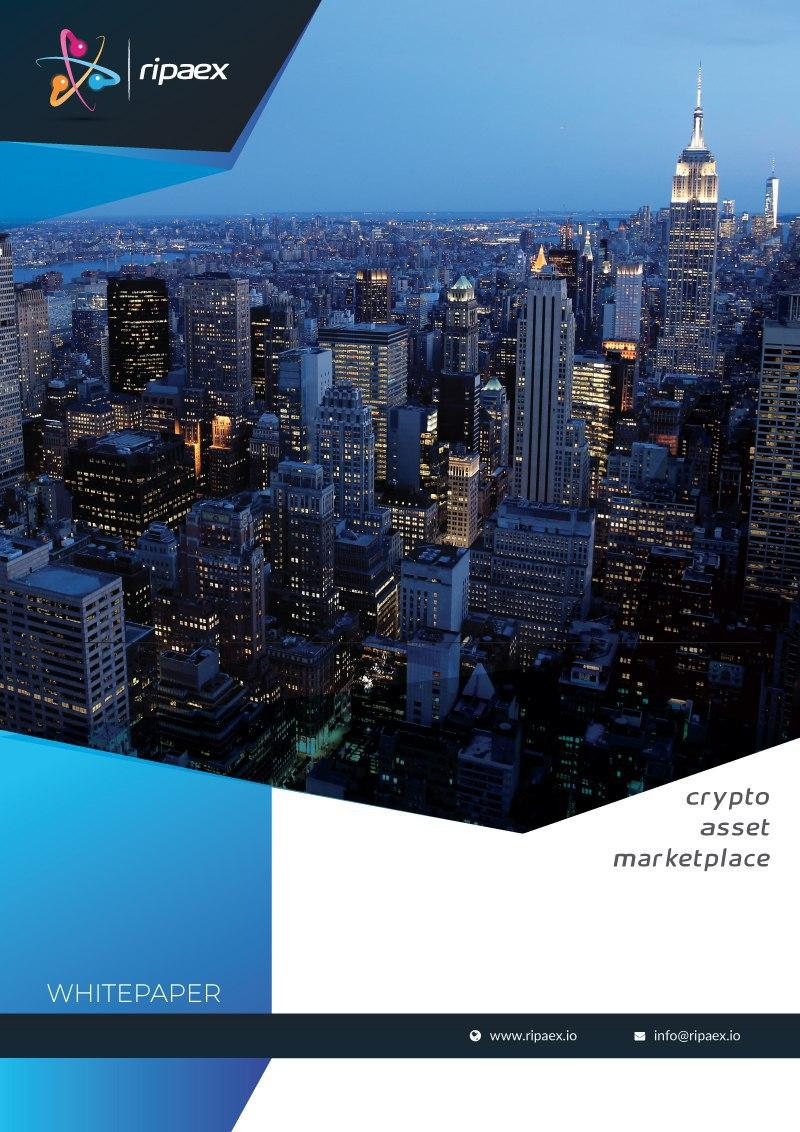
\includegraphics[height=\paperheight]{background}};
\end{tikzpicture}
\endgroup

%----------------------------------------------------------------------------------------
%	COPYRIGHT PAGE
%----------------------------------------------------------------------------------------
\newpage
~\vfill
\thispagestyle{empty}

\noindent Copyright \copyright\ 2018 Ripa Founder Team\\ % Copyright notice

\noindent \textsc{Pubblicato da Ripa Founder Team}\\ % Publisher

\noindent \textsc{www.ripaex.io}\\ % URL

\noindent Materiale protetto dalla Licenza MIT (di seguito la ``Licenza''). Non dovrai usare questo file eccetto in conformità con la Licenza. Puoi ottenere una copia della Licenza a \url{https://opensource.org/licenses/MIT}. A meno che non sia richiesto dalla lagislazione applicata o concordato via scritto, il software distribuito con la Licenza è distribuito \textsc{``così com'è'' senza garanzie di alcun tipo}, esplicite o implicite. Fate riferimento alla Licenza per il linguaggio specifico che governa i permessi e le limitazione indicati dalla Licenza.\\ 

\noindent \textit{Prima pubblicazione, Marzo 2018 - versione 1.0} % Printing/edition date

% \begingroup
% \section{Abstract}\index{Abstract}
% \thispagestyle{empty}
% \addcontentsline{toc}{chapter}{\textcolor{trolleygrey}{Abstract}}
\pagestyle{empty} % No headers
\usechapterimagefalse % If you don't want to include a chapter image, use this to toggle images off - it can be enabled later with \usechapterimagetrue
\chapter{Abstract}

\textbf{Ripa Exchange è un exchange ibrido-decentralizzato con il focus di abbassare il livello di ingresso per aprire 
nuove piattaforme di exchange ed al contempo offrire ai traders un ambiente sicuro ed efficiente per eseguire operazioni di 
trading giornaliere.}\\

Il Team di RipaEx crede che, indipendentemente dagli sviluppi nel mondo delle criptomonete, è oggigiorno costoso per aprire,
gestire, e trovare fiducia nelle proprie operazioni di cambiavaluta virtuale non solo per le risorse richieste per avviare
una piattaforma di scambio affidabile ma soprattutto per sviluppare la piattaforma in sè e trovare la liquidità 
necessaria per generare profitto nei primi 5 anni di attività.\\

Azione è richiesta ed azione è richiesta adesso. Gli utenti sono frustrati da exchange inaffidabili che chiudono scappando con i 
fondi, vengono hackerati oppure non sostengono il carico giornaliero di una'industria crescente come questa è.
Nonostante l'impegno degli imprenditori di exchange per offrire piattaforme di cambio valuta efficienti, affidabili e 
semplici da utilizzare i fondi necessari per costruire queste piattaforme sono nella fascia di 250-300 mila euro senza includere
il costo del personale per offrire supporto di livello platino agli utenti finali, l'infrastruttura di gestione, e costi giornalieri
dell'attività. Tali costi vengono sostenuti per avere una piattaforma di medio livello che per metterla in funzione ci si lega 
ad unica via con una software house per sviluppi futuri.\\

É obbiettivo di questo progetto di sviluppare una piattaforma di cambiavaluta virtuale Open Source, efficiente, affidabile ed 
offrire liquidità\footnote{Grazie alla tecnologia RLSP (Ripa Liquidity Service Provider)} all'exchange così creato dal \textbf{primo}
giorno di attività in modo tale che gli imprenditori in questo settore possono focalizzarsi nel pubblicizzare la propria piattaforma,
offrire supporto tecnico di livello platino ai propri utenti e soddisfare tutte le eterogenee legislazioni nell'industria delle valute virtuali.
Mentre vogliamo che l'esperienza di trading per l'utente finale sia la migliore possibile offrendo un ambiente di trading sicuro ed affidabile.\\
\usechapterimagetrue
% \endgroup

%----------------------------------------------------------------------------------------
%	TABLE OF CONTENTS
%----------------------------------------------------------------------------------------
\chapterimage{chapter_head_1_Beijing.jpg} % Table of contents heading image
\renewcommand*\contentsname{Indice dei Contenuti}
\tableofcontents % Print the table of contents itself
\addcontentsline{toc}{chapter}{\textcolor{trolleygrey}{Indice dei Contenuti}}
\cleardoublepage % Forces the first chapter to start on an odd page so it's on the right
\pagestyle{fancy} % Print headers again
%----------------------------------------------------------------------------------------
%	PART
%----------------------------------------------------------------------------------------


%\part{Part One}

%----------------------------------------------------------------------------------------
%	CHAPTER 2: Introduction
%----------------------------------------------------------------------------------------

\chapterimage{chapter_head_2_London.jpg} % Chapter heading image
\chapter{Introduzione}
Il livello di accesso all'industria delle valute virtuali è piuttosto elevato da un punto di vista tecnico per l'utente medio, 
ed ha un livello di accesso economicamente elevato per l'imprenditore che vuole avviare un'attività in questo campo, valore dato 
dall'acquisto del codice sorgente dell'exchange di criptovalute, dal reclutamento di personale che gestirà l'infrastruttura informatica,
per reclutare operatori di supporto tecnico, per sottostare alle leggi nazionali ed internazionali in materia di AML/KYC, per avere liquidità
dal primo giorno di avvio delle operazioni di cambio. Con questo progetto, Ripa Exchange, vuole abbassare questo livello di ingresso 
perchè \textbf{gestire un exchange è DIFFICILE} ed il Team RipaEx vuole che il lettore e futuro imprenditore nel campo delle valute
virtuali si concentri su cose veramente importanti non cavilli burocratici che l'industria richiede perchè TU vuoi avviare un'attività
in questo campo e tu necessiti del codice sorgente per avviarla, codice sorgente che deve essere concesso gratuitamente alla tua attività.

Per rafforzare questo principio economico il punto è che per avviare un exchange è richiesto un investimento esiguo dal tuo 
venture capital di riferimento e anche con un tale investimento il ritorno dei fondi investiti all'angel investor non sono garantiti
nei primi 5 anni di attività.

Per avviare un servizio professionale di cambiavaluta virtuale crediamo che il codice sorgente dell'exchange e la liquidità da offrire ai tuoi clienti
dal primo giorno di attività dovrebbero esserti forniti gratuitamente: non deve essere accettabile pagare \euro150.000,00 ad una software house
solo per avere una piattaforma che funzioni e per la quale dovete erogare altri \euro100.000,00-150.000,00 per brandizzarla, personalizzarla
per i vostri scopi legandovi in questo modo ad una singola software house che potrebbe fallire in futuro e che vi farebbe ritrovare
senza poter fare ulteriori modifiche al vostro exchange in quanto non vi hanno mai consegnato il codice sorgente della piattaforma
su cui il vostro business fa affidamento.

\textbf{Noi crediamo che tutto questo debba essere gratuito}: dobbiamo offrirti la miglior tecnologia nel mercato attuale in modo tale che tu 
possa focalizzarti sulla tua attività mentre noi ci focalizziamo in sviluppare la tecnologia per gestire la tua attività in maniera efficiente, 
sicura, responsiva e produttiva. Questo è il motivo per cui RipaEx si prefigge lo scopo di sviluppare una rete di exchange
focalizzandosi su di un'architettura che è \textit{efficiente, sicura, responsiva, compliant e personalizzabile} in modo tale che ogni exchange
nella rete può basarsi su di fondamenta solide mentre è comunque possibile modificare la singola istanza secondo le personalizzazioni 
che la compagnia che gestisce quell'istanza richiede.

Per raggiungere questo scopo abbiamo scelto di sviluppare la tecnologia Ripa Liquidity Service Provider basata su ARK - a blockchain for consumer adoption - 
il cui obbiettivo primario è incrementare l'adozione delle tecnologie blockchain agli utenti finali focalizzandosi su due aree critiche: 
\underline{Una Efficiente e Sicura Tecnologia di Base} e \underline{Servizi Reali per Gente Comune}. L'ecosistema ARK è ancora ad uno stadio
iniziale di sviluppo: la futura implementazione di ARK 2.0 permetterà di eseguire smart contract nativi sulla blockchain, che permetteranno
alla blockchain ARK di competere con la sua concorrente Ethereum da un punto di vista tecnologico. RLSP permetterà a tutti gli exchange della rete Ripa
di scambiare liquidità condividendo lo stesso libro degli ordini in base ai parametri di condivisione della singola istanza dell'exchange Ripa
configurabili nella tua area amministratore.

Il Ripa Founder Team (RFT), come presentato in ripaex.io, opera nel nome del gruppo Ripa. L'RFT è responsaile per l'uso corretto dei finanziamenti
ottenuti nella campagna di scambio token RIPA TEC come spiegato di seguito in questo documento.

Il RFT dispone che i fondi delle fasi di PreSale e RIPA TEC saranno usati esclusivamente per il finanziamento del progetto 
\emph{RipaEx} come spiegato in questo whitepaper, che saranno resi disponibili per estrazione nella piattaforma apposita resta disponibile
più tardi quest'anno tec.ripaex.io, e che dovranno risultare nella creazione di una entità legale che sarà chiamata \emph{RipaEx}. La creazione di tale 
compagnia è pianificata per il primo quadrimestre del 2019.

Fino a tale data RFT opera invece di \emph{RipaEx, una compagnia nel processo di essere incorporata}.

\section{Terminologia}\index{Terminologia}
\begin{description}
	\item[\textsc{Ripa Exchange:}] un exchange FIAT $\Leftrightarrow$ CRYPTO sviluppato partendo dal codice sorgente di Peatio \cite{peatio}
	\item[\textsc{Ripa Blockchain:}] una blockchain DPOS in cui la liquidità ed il libro mastro degli ordini sono condivisi tra tutti gli exchange della rete
	\item[\textsc{Ripa Token - XPX:}] un token crittograficamente sicuro tramite il protocollo DPOS scambiato sulla blockchain Ripa 
	\item[\textsc{RIPA:}] l'ecosistema finanziario DPOS composto da Ripa Exchange e Ripa Blockchain
	\item[\textsc{RIPAEX:}] il nome del progetto, sito web del progetto e domini del progetto
	\item[\textsc{RLSP:}] Ripa Liquidity Service Provider, un libro ordini condiviso tra gli exchange nella stessa rete Ripa
	\item[\textsc{RipaEx ICO:}] il nome del periodo di cambiavaluta a tasso fisso composto dalle fasi di PreSale e RIPA TEC	
	\item[\textsc{ARK:}] una piattaforma per l'adozione consumer di tecnologie blockchain \cite{ark}
	\item[\textsc{ACES:}] Ark Contract Execution Services \cite{aces} fornisce semplici protocolli e strumenti per costruire robusti
	mercati di scambio tra blockchain basati sulla tecnologia ARK SmartBridge
	\item[\textsc{``,'' o ``.'':}] la notazione italiana per virgola decimale e punti di migliaia è stata scelta per la stesura di questo 
	whitepaper: detto questo “,” rappresenta un punto decimale e “.” rappresenta la separazione tra migliaia e multipli di migliaia 
\end{description}

%\pagebreak
\section{Roadmap}
Saranno percorse essenzialmente quattro fasi del progetto RipaEx:
\tcbset{roadmapBox/.style={colback=yellow!10!white,colframe=azure(colorwheel),
equal height group=nobefaf,width=(\linewidth-1pt), height from=4cm to 8cm, nobeforeafter,
	center title,
	valign=top, halign=left}}
\begin{center}
\begin{tcolorbox}[roadmapBox,
	title=\textbf{\textsc{Finanziamneto del progetto: XPX presale e RIPA TEC (WP2)}}]

	Questa fase riconosce l'esistenza di un interesse in questo sviluppo di mercato
	da un capo del Mondo all'altro in riguardo l'abbassamento del livello economico di ingresso
	per sviluppare exchange di criptovalute.
	L'obbiettivo è di eseguire la prima analisi omnicomprensiva dello stato dell'arte per fondare
	le basi delle fasi sucessive del progetto e per sviluppare il primo prototipo
	funzionante di un exchange centralizzato con il codice di Peatio.\\
	\vspace{1cm}
	\centering\textbf{\textsc{Prevista fine della fase: Gennaio 2019}}.
\end{tcolorbox}
\resizebox{0.05\textwidth}{26pt}{$\Downarrow$}
\begin{tcolorbox}[roadmapBox,
	title=\textbf{\textsc{Apertura del primo exchange e sviluppo di strumenti e risorse (WP3)}}]

	La seconda fase prende i risultati della prima e sviluppa da qui
	una serie di strumenti e risorse che offrono guida concisa ed omnicomprensiva per 
	i player senza considerare lo Stato di incorporazione/sviluppo del progetto. Con la prima
	istanza di Ripa Exchange in esecuzione/aperta al pubblico i primi contatti con altri player economici
	nell'industria delle valute virtuali possono essere presi.\\
	\vspace{1cm}
	\centering\textbf{\textsc{Prevista fine della fase: Giugno 2019}}.
\end{tcolorbox}
\resizebox{0.05\textwidth}{26pt}{$\Downarrow$}
\begin{tcolorbox}[roadmapBox,
	title=\textbf{\textsc{Esecuzione, diffusione (WP 7/8) e Coordinamento del Progetto (WP1)}}]

	Durante tutta la durata del progetto,
	attività di diffusione (WP 7/8) sono eseguite nelle quali i risultati dei singoli
	pacchetti di lavoro individuali sono consegnati ai relativi gruppi obbiettivo inclusi
	partners del progetto, investitori RipaEx, manager di exchange, partner bancari come anche
	tutti gli altri gruppi obbiettivo rilevanti al progetto RipaEx in esecuzione.
	Questa fase copre una vasta scala di tecniche di diffusione, da libri stampati ed 
	elettronici, a workshop e sessioni di training, hackatons, tutti aventi 
	come obbiettivo di definire standard per la comunicazione tra exchange gestiti da entità 
	pubbliche e private nell'industria delle valute virtuali.
	Un pacchetto di lavoro globale riguardante la gestione del progetto dall'inizio alla fine, 
	assicurando coordinazione adeguata, quality assurance e controllo del budget (WP1).
\end{tcolorbox}
\resizebox{0.05\textwidth}{26pt}{$\Downarrow$}
\begin{tcolorbox}[roadmapBox,
	title=\textbf{\textsc{Sviluppo di un exchange ibrido-decentralizzato (WP 4-6)}}]

	Usando gli strumenti e le risorse sviluppate in WP3, il pacchetto di lavoro 4-6
	si focalizza di mettere in pratica la conoscenza acquisita e gli strumenti. I tre
	pacchetti di lavoro riflettono tre punti focali (e gruppi target) nel network di 
	exchange creato per installare demo di successo su scala locale, nazionale ed internazionale:
	l'incorporazione di istanze di Ripa Exchange locali (WP4), analisi tecnica della tecnologia
	Ripa Liquidity Service Provider (WP5), e primo MVP dell'exchange ibrido decentralizzato (WP6).
	La fase demo dal cuore dell'azione RipaEx; WP 2 e 3 focalizzano in produrre consegne (ad esempio
	strumenti) che abilitano attività di produzione demo efficienti e di successo.\\
	\vspace{1cm}
	\centering\textbf{\textsc{Prevista fine della fase: Gennaio 2021}}.
\end{tcolorbox}
\end{center}

\section{RipaEx Partners - RipaEx Governance}\index{RipaEx Partners - RipaEx Governance}
La maggior parte dei parnter sono imprenditori nell'industria delle valute virtuali, tuttavia
un Istituto di Ricerca ed Organizzazioni Finanziari sono anche presenti. I partner sono:
\begin{itemize}
	\item \textbf{Coordinatore}: RipaEx SCIC 
	\item \textbf{CoBeneficiari}: Ripa Exchange Ltd \todo{TODO: AGGIUNGERE PARTNER RIPAEX}
\end{itemize}

\subsection{RipaEx Governance}\index{RipaEx Governance}
La creazione di nuovi exchange nella rete Ripa, il rilascio dei fondi dell'RCF per la creazione di nuovi exchange saranno decise
su votazione maggioritaria dei delegati della rete Ripa. Le modifiche del singolo exchange, invece, saranno appannaggio 
esclusivo della compagia che gestisce la singola istanza dell'exchange.

Il progetto RipaEx si incorporerà come società di interesse collettivo per profitto appena la rete Ripa sarà stabile, mentre Ripa Exchange Ltd
società a gestione della prima istanza di exchange in esecuzione sarà incorporata come compagnia privata nel primo quarto
del 2019.

\section{Sommario del Progetto}
\begin{enumerate}
	\item \textbf{\textsc{cosa}}: RipaEx è un progetto per facilitare la presa di standard per condividere liquidità tra mercati di asset
	criptosicuri (crypto asset marketplace).
	L'obbiettio di RipaEx è la promozione di codice sorgente condiviso per portafogli ed exchange nell'industria delle valute
	virtuali: è obbiettivo di questo documento di riferimento di dare informazioni dettagliate per futuri
	sviluppatori di exchange oppure futuri imprenditori in questo campo, per abilitare processi di decision-making corretti e per 
	assicurare il successo dei loro progetti proposti.
	Il progetto RipaEx si prefigge l'obbiettivo di analizzare il potenziale reale di applicazione nel Paese scelto 
	di una rete di exchange e la sua posizione nel mercato.
	\item \textbf{\textsc{cosa}}: gli asset crittograficamente sicuri (aka: ``crypto assets'') sono un'alternativa agli asset emessi dalle borse
	valori dei vari Paesi che ne possiedono una. Anche se, tuttavia, molte borse valori mondiali danno la possibilità ai loro 
	utenti di verificare e gestire gli asset in loro possesso il processo non è sempre trasparente e/o semplice e questo è il motivo 
	per cui a partire dal 2009 \cite{bitcoin} un nuovo tipo di asset (verificabile dalla comunità) è stato implementato
	per dare a piccoli, medi e grandi investitori completa trasparenza nella gestione dei loro asset di investimento.
	\item \textbf{\textsc{quanto}}: recenti sviluppo a livello dell'Unione Europea e globalmente stanno trasformando sia come le valute virtuali
	sono trattate sia il modo in cui le ICO (Initial Coin Offering) sono legislate. Questi sviluppi combinati hanno messo
	l'uso e la produzione di valute virtuali in una luce favorevole in costante ascesa. \\
	In Ottobre 2015 la Corte Europea di Giustiza ha sentenziato che bitcoin ed altre valute virtuali sono esenti dalla tassazione IVA. \\
	In Luglio 2016 la Commissione Europea ha adottato proposal per ammendare la legislazione vigente 4th Anti-Money Laundering Directive (4AMLD) 
	che introduca le figure degli exchange di valute virtuali ed offritori di wallet all'interno del framework europeo di adeguata verifica
	dell'utente ed antiriciclaggio \cite{EUAMLCrypto}.\\
	In Febbraio 2018 la Commissione Europea lancia l'Osservatorio EU sulle Blockchain (EU Blockchain Observatory and Forum) \cite{EUBOaF} 
	per osservare gli sviluppi chiave nella tecnologia blockchain, promuovere attori europei e rafforzare l'ingaggio europeo con
	diversi stakeholders coinvolti in attività correlate alla blockchain.
	\item \textbf{\textsc{perchè}}: c'è ancora poca regolamentazione sulle ICO e solo gli Stati Uniti d'America al momento
	hanno scritto una legislazione definendo i token delle ICO come securities \cite{SECICO}.
	\item \textbf{\textsc{chi}}: i risultati delle indagini di mercato indicano che il medio tech savvy dai 18 ai 45 anni di età è
	l'utente medio delle valute virtuali tuttavia compagnie in finanza stanno anche comincianto ad inserire schemi di 
	valute virtuali all'interno dei loro portafogli specialmente dalla presentazione del contratto bitcoin futures 
	da parte del Gruppo CME Group Inc. nella borsa valori di Chicago lo scorso 18 Dicembre 2017.
	\item \textbf{\textsc{quanto}}: la capitalizzazione di mercato totale dell'industria delle valute virtuali è stata stimata attorno
	ai 317 miliardi di USD \footnote{Dati Coinmarketcap Aprile 2018}
	ed è prevista la crecita a 5.000 miliardi di USD nel prossimo timeframe di 10 anni \cite{cryptoMCTenYears}.
	\item \textbf{\textsc{dove}}: autorità locali stanno lavorando con i Governi Nazionali per essere certi che gli exchangers sul 
	territorio nazionale di riferimento seguono le procedure nazionali ed internazionali di AML/KYC.
	Venture Capital ed Angel Investors stanno cominciando a rilasciare soluzioni di finanziamento a start-up nell'industria delle
	valute virtuali - FinTech in tutto il mondo, dall'America all'Asia passando per l'Europa ed alcuni Paesi
	stanno avviando schemi di valuta virtuale statali per testare lo scambio di beni e servizi sulle tecnologie a libro 
	mastro condiviso (DLTs - Distributed Ledger Technologies) \cite{petro}.
	\item \textbf{\textsc{quanto costa}}: il costo medio per avviare il proprio crypto assets marketplace è attorno a \euro 150.000,00, 
	al pagamento di tale somma avrete unicamente un'istanza in esecuzione della vostra piattaforma di cambio: al suddetto prezzo dovete aggiungere i costi
	di personalizzazione della piattaforma prima del lancio ed in futuro, pubblicizzazione della piattaforma, costo di gestione dei server, 
	amministratori di rete, operatori del centro di supporto e costo del dipartimento legale per seguire le leggi AML/KYC dello Stato
	in cui avete deciso di incorporare il vostro exchange e per gestire l'amministrazione della compagnia dietro di esso.\\
	\textbf{Questi costi nascosti sono la ragione per cui noi di RipaEx riteniamo che possedere il codice sorgente del proprio exchange è il miglior
	modo per avviare e mantenere un'attività in questa industria}.
	\item \textbf{\textsc{come}}: il problema principale nell'eseguire un'operazione di cambio FIAT $\Leftrightarrow$ CRYPTO è di trovare partner bancari affidabili
	e nel seguire le differenti procedure AML/KYC del Paese o dei paesi di incorporazione.
	\item \textbf{\textsc{cosa}}: le operazioni di cambio valuta virtuale classiche sono le seguenti:
		\begin{itemize}
			\item \textbf{scambio ad una-via}: nella quale un'applicazione centralizzata ha tutta la liqudità da offrire ai potenziali utenti
			\item \textbf{scambio a due-vie}: nella quale un exchange centralizzato o decentralizzato accoppia richiesta di vendita con richiesta di aquisto degli utenti
		\end{itemize}
		Dalla classificazione data sopra una ulteriore sotto-classificazione è d'obbligo:
		\begin{itemize}
			\item \textbf{scambio FIAT $\Leftrightarrow$ CRYPTO}: nella quale lo scambio avviene tra valuta FIAT\footnote{Valute emesse dalle banche centrali: EUR, USD, GBP, JPY, altre...}
			e valuta virtuale
			\item \textbf{scambio CRYPTO $\Leftrightarrow$ CRYPTO}: nella quale lo scambio avviene tra valuta virtuale e valuta virtuale
		\end{itemize}
	Dalle quattro classificazioni sopra si può costruire una matrice con quattro possibili configurazioni per sviluppare la piattaforma di cambia valuta virtuale
	che preferite.
	\begin{tcbraster}[raster columns=3,raster rows=1,raster height=0.8cm,
		valign=center, halign=center,
		enhanced,size=small,sharp corners,colframe=azure(colorwheel),coltext=white,
		colback=azure(colorwheel),fit algorithm=hybrid* ]
		\tcboxfit{}
		\tcboxfit{\textbf{una-via}}
		\tcboxfit{\textbf{due-vie}}
	\end{tcbraster}
	\begin{tcbraster}[raster columns=3,raster rows=2,raster height=5cm,
		valign=center, halign=center,
		enhanced,size=small,sharp corners,colframe=silver,coltext=black,
		colback=silver,fit algorithm=hybrid* ]
		\tcboxfit{\textsc{\textbf{FIAT $\Leftrightarrow$ CRYPTO}}}
		\tcboxfit{\tcbfontsize{0.8} applicazione di acquisto veloce}
		\tcboxfit{\tcbfontsize{0.8} exchange con partnership bancaria}
	
		\tcboxfit{\textsc{\textbf{CRYPTO $\Leftrightarrow$ CRYPTO}}}
		\tcboxfit{\tcbfontsize{0.8} applicazione di scambio veloce}
		\tcboxfit{\tcbfontsize{0.8} exchange senza partnership bancaria}
	\end{tcbraster}	

	\item \textbf{\textsc{con cosa}}: le specifiche da guardare quando scegliere la propria piattaforma di exchange sono le seguenti: 
		\begin{enumerate}[label*=\arabic*.]
			\item \textbf{Codice}: Open Source, Closed Source oppure soluzione ibrida
			\item \textbf{Modularità}: separazione tra l'engine di cambio (engine di accoppiamento ordini), la UI e l'anagrafica utenti
			\item \textbf{Responsività della UI}: la UI deve essere responsiva su tutti i device (desktop e mobile)
			\item \textbf{Conformità}: con gli standard industriali correnti e con la legislazione vigente
			\item \textbf{Personalizzazione}: dell'engine di cambio, delle valute da offrire, della UI e di altri aspetti della piattaforma di cambio
			\item \textbf{Sicurezza} dei fondi nell'exchange: possibilità di configurare il salvataggio dei fondi in cold wallet e hot wallet
			\item \textbf{Trasparenza} dei fondi: proof of solvency dell'exchange
			\item \textbf{Multi-Accounts trading}: possibilità di configurare facilmente nuovi mercati da offrire agli utenti
			\item \textbf{Multi-Accounts users}: possibilià di loggarsi nella piattaforma tramite Google, Facebook, Twitter, e conformità
			con gli standard della FIDO Alliance per le credenziali personali
		\end{enumerate}	
	\textbf{Queste non sono solo decisioni tecniche da prendere ma anche economiche} specialmente il possesso o meno del codice sorgente della propria 
	piattaforma	crypto asset marketplace per permettere le future personalizzazioni del proprio exchange in maniera indipendente invece di affidarsi
	ad una singola software house che esegua le personalizzazioni per voi.
	\item \textbf{\textsc{come}}: possibili operazioni per trovare nuovi utenti per le vostre operazioni di cambia valuta virtuale sono:
	campagne di marketing ``ad hoc'', funzionalità innovative nell'industria, livelli di tassazione del trading basati sulla quantità, 
	bonus di registrazione e per quantità di scambiato giornaliero/settimanale/mensile, marketing affiliato per gli utenti che portano
	amici a scambiare nell'exchange.
	\item \textbf{\textsc{come}}: per incorporare una crypto asset marketplace un progetto deve tenere in considerazione la seguente legislazione:
		\begin{itemize}
			\item \textbf{AML/KYC}: \textit{Fourth Anti-Money Laundering Directive} se l'attività viene avviata nell'Unione Europea \cite{4AMLD} 
			oppure la legge AML/KYC di riferimento nel Paese di incorporazione (ad esempio \textit{Intelligence Reform \& Terrorism Prevention Act of 2004}
			emessa dalla FinCEN per incorporazione negli Stati Uniti d'America).\\
			Raccomandazioni internazionali per eseguire verifiche AML/CFT sono data dalla Financial Action Task Force on Money Laundering \cite{FATF}.
			\item \textbf{Licenza di Pagamento}: l'attività decisamente più ardua in riguardo alla legittimazione delle operazioni di cambio FIAT $\Leftrightarrow$ CRYPTO
			è l'ottenimento di una \textit{Licenza PSD} \cite{PSD}.
			La licenza PSD seguen la Direttiva del Concilio Europeo 2007/64/EC ed è applicata in ogni Paese attraverso le sue leggi nazionali.
			Il costo di una licenza PSD può variare da centinaia di migliaia di euro ad un ordine di grandezza superiore al seconda del volume di affari.
		\end{itemize}
	\item \textbf{\textsc{chi}}: la natura dell'attività in considerazione del progetto RipaEx 
	(una rete di piccoli exchange FIAT $\Leftrightarrow$ CRYPTO)
	implica che ogni exchange debba avere uno staff di 7-8 persone: N.2 sviluppatori, N.1 operatore di rete/sicurezza, 
	N.1 commerciale amministrativo, N.2 operatori di supporto tecnico, N.1 legale e consigliere sulla tassazione. \\
	Il turnover di una tale compagnia tuttavia, considerato l'alto valore aggiunto del prodotto scambiato, e possibile che raggiunga cifre
	superiori ad \euro 350.000 annui e possibilmente di un'ordine di grandezza superiore. Un'attività di questa dimensione
	suggerisce automaticamente le possibili forme societarie: una ditta individuale, una società a responsabilità limitata,
	una società non-profit o attività sociale, una cooperativa gestita dagli amministratori delegati dei vari exchange.
	Le Agenzie Finanziarie sono attori fondamentali nell'indicare questa scelta, tuttavia la tipologia di attività da
	incorporare dipende dallo status legale che si vuole dare alla stessa e questo varia da Paese a Paese.		
	\item \textbf{\textsc{come}}: una risorsa di fondi per una marketplace di dimensioni piccole-medie può essere: prestito bancario,
	prestito privato a basso interesse, credito commerciale, equity finanziario, venture capital di business angels. Avendo un
	business plan consolidato e garanzie finanziarie adeguate sono elementi chiave nell'assicurarsi i finanziamenti necessari
	allo sviluppo che si vuole eseguire. Il Fondo Europeo di Investimento (EIF) della Banca di Investimento Europea (EIB)
	offre supporto nella forma di garanzia per le SME (piccole e medie imprese).
	\item \textbf{\textsc{chi}}: gli argomenti per l'incorporazione di un crypto asset marketplace sono la libertà finanziaria, la
	decentralizzazione delle operazioni di trasferimento del valore ed il reale possesso del proprio denaro.
	Ci sono altri benefici, ben documentati, come pagamenti veloci, guadagno a lungo termine dato da un'economia deflazionaria, previsione
	delle depressioni economiche come quella del 2008, ma soprattutto le valute virtuali sono l'unico competitor diretto alle operazioni
	di trasferimento del valore centralizzate eseguite dalle banche centrali.
	\item \textbf{\textsc{perchè}}: c'è consenso in letteratura che l'uso delle valute virtuali invece delle valute fiat permette un livello di
	libertà finanziaria maggiore specialmente perchè queste tecnologie di trasferimento valore rientrano nella scuola
	di economia Austriaca \cite{austrianTheory} secondo molte fonti \cite{misesItalia} anche se tuttavia bitcoin dà il meglio come
	mezzo di scambio e mancherebbe della stabilità di tasso di cambio che la renderebbero una riserva di valore accettabile.
	\item \textbf{\textsc{perchè}}: benefici delle tecnologie di valuta virtuale come bitcoin sono in una economia deflazionistica,
	in un'emissione limitata di valuta, in trasferimenti di valore pressochè istantanei e senza barriere statali, in 
	relativo anonimato e nella separazione tra entità che producono la moneta (miner) ed entità che definiscono la teoria monetaria
	alla base della stessa (sviluppatori).
	\item \textbf{\textsc{come}}: securizzare asset sulla blockchain significa semplicisticamente eseguire le tre operazioni
		\begin{enumerate}[label*=\arabic*.]
			\item \textbf{Generazione di una chiave privata casuale}
			\item \textbf{Conversione della chiave privata generata in (1) in una chiave pubblica}: un protocollo comune per la conversione
			in questa industria è l'algoritmo ECDSA
			\item \textbf{Conversione della chiave pubblica generata in (2) in un indirizzo di valuta}: protocolli comuni per eseguire questa
			conversione sono le funzioni hash SHA-256, Base58 encoding, Base32 encoding
		\end{enumerate}
	A questo punto qualsiasi valore inviato all'indirizzo generato in (3) è garantito dalla doppia spesa nella blockchain scelta ed accessibile
	solo dal possessore della chiave privata generata in (1).
	\item \textbf{\textsc{dove}}: due fattori critici che interessando l'industria delle valute virtuali sono la concorrenza bancaria ed il 
	banning a livello statale. Anche se l'armonizzazione delle leggi europee in materia sarà di beneficio all'industria sia in termini di 
	tassazione sia in termini di garanzia per l'utilizzatore finale, al momento questo ancora non avviene. Ogni Paese su scala mondiale 
	ha la propria legislazione in materia ed i propri regimi di tassazione per tutte le operazioni di cambiavaluta virtuale,
	il banning statale invece va da livelli	di permissività totale come nell'Unione Europea al banning totale con 
	imprigionamento come in Bangladesh \cite{bitcoinLegality}. 
	\item \textbf{\textsc{dove}}: i paesi asiatici della Corea del Sud, Cina e Giappone sono sempre stati leader nell'industria delle valute virtuali
	negli ultimi 9 anni con un approccio proattivo in materia di tassazione. All'inizio del 2017 in Giappone il bitcoin è stato 
	dichiarato legal tender tuttavia in Cina recentemente sono state dichiarate illegali tutte le operazioni di cambiavaluta virtuale ed ICO 
	e gli exchange nel Paese asiatico stanno cessando le loro attività di cambio. 
	\item \textbf{\textsc{dove}}: qualsiasi valutazione del mercato locale dovrebbe comprendere: numero di potenziali utenti, tipo di exchange da 
	incorporare (FIAT $\Leftrightarrow$ CRYPTO oppure CRYPTO $\Leftrightarrow$ CRYPTO), tipi di protocolli da integrare (POW, DPOS, Masternode, altri...), 
	tipi di servizi da offrire (trading, trading avanzato, processore di pagamento, altri...), se l'exchange incorporato è di tipologia
	FIAT $\Leftrightarrow$ CRYPTO numero e tipologia di processori di pagamento accettati (PayPal, OKPAy, MoneyPolo, altri...), numero di exchange
	simili nella regione di incorporazione. 
	\item \textbf{\textsc{chi}}: ci sono numerose opzioni per offrire una polizza assicurativa sui fondi degli utilizzatori finali (Customer Protection):
	creare comprensione tra gli utenti che il possesso delle chiavi private dei fondi mette loro in \textbf{posizione di responsabilità} 
	nei confronti di un'eventuale perdita dei fondi, in quanto nessuno può recuperare le chiavi private una volta che sono perse. 
	Creare comprensione negli utenti per non lasciare i fondi negli exchange ("\textit{Be Your own Bank!!}"), lasciandogli scegliere a quale
	exchange del mercato affidarsi.
	\item \textbf{\textsc{chi}}: mentre è decisamente costoso assicurare la valuta e le operazioni di trasmissione del valore, esempi di customer protection
	in questa industria sono: la piattaforma Kraken ha recentemente permesso agli utenti Mt. Gox di richiedere rimborso tramite
	la loro piattaforma, l'exchange BitFinex ha emesso token BFX per ripagare i propri utenti della perdita di 120.000 bitcoin (pari a circa \$72.000.000
	all'epoca dell'hacking) dovuti al cambio del livello di sicurezza dell'exchange stesso, Ethereum ha eseguito uno fork al blocco 1920000
	per ovviare ad un bug nel codice della Decentralized Autonomous Organization che ha permesso la sottrazione di \$50.000.000 di ETH dallo smart contract
	di The DAO, altri casi di hacking...
	\item \textbf{\textsc{Raccomandazioni finali/conformità legislativa}}: se intendete incorporare un exchange 
	FIAT $\Leftrightarrow$ CRYPTO dovete focalizzarvi in prima istanza nella conformità legislativa in materia 
	di AML/KYC nel Paese di incorporazione, le fondazioni
	bitcoin locali possono aiutarvi in focalizzare le vostre operazioni di cambio basate sugli interessi degli utilizzatori finali 
	nel Paese di incorporazione, promuovendo ambienti \textit{cryptocurrency friendly} nell'area di interesse.
\end{enumerate}


%----------------------------------------------------------------------------------------
%	CHAPTER 3: Ripa Exchange
%----------------------------------------------------------------------------------------

\chapterimage{chapter_head_3_Singapore.jpg} % Chapter heading image

\chapter{L'Exchange Ripa}
Ripa Exchange è un crypto asset marketplace implementato seguendo i più avanzati standard industriali seguendo il principio
``\textit{open source, sicuro ed efficiente}''. Ripa Exchange si prefigge di servire come piattaforma sicura, UI responsive, 
personalizzabile, facile da usare per gli imprenditori in questo settore abbracciando i principi Open Source e la fiducia pubblica.\\\\
Ripa Exchange è implementato utilizzando il framework Ruby on Rails ed altre tecnologie all'avanguardia e sarà migrato verso
un exchange ibrido-decentralizzato dove tutti gli exchange nella rete Ripa condivideranno la stessa liquidità grazie alla tecnologia R.L.S.P..

\section{Mission}
\begin{quotation}
	``\textit{La nostra mission è di costruire il crypto asset marketplace migliore al mondo con un trading engine ad alte prestazioni 
	e sicuro abbastanza da poter essere utilizzato dagli utenti in tutta fiducia. In aggiunta vogliamo far fare un passo avanti 
	alla tecnologia degli exchange di criptomonete offrendo supporto tecnico e nuove funzionalità. Aiutiamo persone da tutto il mondo
	alla costruzione dei loro exchange personalizzati.}''
\end{quotation}

Il supporto tecnico è sempre apprezzato: sentitevi liberi di inoltrare pull-request oppure aprire issue nei nostri 
\href{https://github.com/RipaEx}{repository GitHub}.

\section{Funzionalità}
Un libero, trasparente ed internazionalizzato exchange di criptomonete open source.

\tcbset{featureBox/.style={colback=yellow!10!white,colframe=white!20!black,
equal height group=nobefaf,width=(\linewidth-1pt)/3, height=5.0cm, nobeforeafter,
	center title,
	valign=top, halign=left}}
\begin{tcolorbox}[featureBox,
	title=\textsc{Open Source} \faCircleONotch]

	\small	Tutto il codice sorgente prodotto è rilasciato sotto licenza MIT.\\\vspace{5mm}
	\tiny Ripa Exchange è un'architettura di cambiavaluta virtuale personalizzabile che connette semplicemente procedure
	di autentificazione AML/KYC, report ETL ed altri servizi.
\end{tcolorbox}
\begin{tcolorbox}[featureBox,
	title=\textsc{Conforme} \faCheck]

	\small Standard internazionali AML/KYC.\\\vspace{5mm}
	\tiny La KYC di Ripa Exchange permette procedure KYC semplici a livello bancario e conformi ai requisiti di 
	Customer Due Diligence (CDD).
\end{tcolorbox}
\begin{tcolorbox}[featureBox,
	title=\textsc{Trasparente e Configurabile} \faCogs]

	\small Personalizza a tuo modo\\\vspace{5mm}
	\tiny Le principali funzionalità sono state racchiuse nel codice sorgente: registrazione pulita ed 
	interfaccia di login semplice, procedure di deposito e prelievo personalizzate, miglior accoppiamento di ordini 
	di vendita ed acquisto, altro... . Queste funzionalità sono già integrate nell'exchange finale e sono pronte all'uso
	senza lavoro aggiuntivo. 
\end{tcolorbox}

\begin{tcolorbox}[featureBox,
	title=\textsc{Internazionalizzazione} \faLanguage]

	\small	Gli utenti possono visualizzare Ripa Exchange nella lingua preferita.\\\vspace{5mm}
	\tiny Supportando diversi linguaggi comuni, Ripa Exchange rende facili le operazioni di trading degli utenti
	nella loro lingua madre. Vi incoraggiamo a contribuire alla varietà linguistica di Ripa Exchange: la comunità
	di utenti trarra beneficio da questa.
\end{tcolorbox}
\begin{tcolorbox}[featureBox,
	title=\textsc{Prova di Solvibilità} \faUsers]

	\small	PoS facilmente rilasciabile.\\\vspace{5mm}
	\tiny La Prova di Solvibilità (PoS) di Ripa Exchange permette agli utenti di verificare la solvibilità dell'exchange
	senza compromettere la privacy del singolo utente.
\end{tcolorbox}
\begin{tcolorbox}[featureBox,
	title=\textsc{Multi-Accounts Trading} \faHandSpockO]

	\small	Facilità di configurazione delle valute.\\\vspace{5mm}
	\tiny Ripa Exchange permette di creare molteplici account e scambiare in diverse valute: quest operazione è
	di facile esecuzione in Ripa Exchange.
\end{tcolorbox}

\begin{tcolorbox}[featureBox,
	title=\textsc{Multi-Accounts Utenti} \faSuitcase]

	\small	Facilità di configurazione degli account utente.\\\vspace{5mm}
	\tiny Ripa Exchange offre molteplici tipologie di login utente tramite Google, Facebook, Twitter ed segue
	gli standard FIDO Alliance per la sicurezza degli account.
\end{tcolorbox}
\begin{tcolorbox}[featureBox,
	title=\textsc{Exchange Enterprise} \faInstitution]

	\small Avvio piccolo, crescita grande.\\\vspace{5mm}
	\tiny Ripa Exchange offre funzionalità enterprise incluso un matching engine ad alte prestazioni, 
	thread di lavoro distribuito scalabili ed autentificazione a due fattori tramite SMS.
\end{tcolorbox}
\begin{tcolorbox}[featureBox,
	title=\textsc{Funzionale ed Intuitivo} \faIntersex]

	\small	Per il trader novizio, per il trader esperto.\\\vspace{5mm}
	\tiny Interfaccie di registrazione, login e trading pulite. Procedure di deposito e prelievo personalizzate 
	e prova di solvibilità integrata.
\end{tcolorbox}

\section{Analisi Funzionale}
\todo{TODO: scrivere analisi funzionale}
\begin{enumerate}
	\item \textsc{Cosa serve Redis-RabbitMQ}:
	\item \textsc{Cosa serve NodeJS}: 
	\item \textsc{Cosa serve Pusher}:
	\item \textsc{ER MySQL}:
	\item \textsc{Ruby gerarchia directory}:
\end{enumerate}

\section{Stack Tecnologico}
\todo{TODO: scrivere più in dettaglio questa sezione}
\begin{itemize}
	\item \textbf{\textsc{Ruby on Rails}}:
	\item \textbf{\textsc{MySQL}}: 
	\item \textbf{\textsc{Redis}}:
	\item \textbf{\textsc{RabbitMQ}}:
	\item \textbf{\textsc{NodeJS}}:
	\item \textbf{\textsc{Pusher}}:
\end{itemize}

\section{Interfaccia Utente}
La user interface di Ripa Exchange è basata sulla user interface di Peatio una UI responsiva sviluppata in Ruby on Rails e 
completamente separata dall'engine ordini dell'exchange.
Il design per una UI personalizzata sono in corso per offrire agli utenti Ripa Exchange la miglior esperienza utente in ogni
dispositivo: in questa sezione potete trovare alcuni screenshot della UI attuale dell'exchange.

\subsection{Interfaccia End-User}
Di seguito alcuni screenshot dell'interfaccia utente end-user dell'exchange Ripa:
\textcolor{darkred}{questi screenshot sono un lavoro in corso e non è detto che rappresentino l'interfaccia utente del prodotto finale}
\begin{center}
	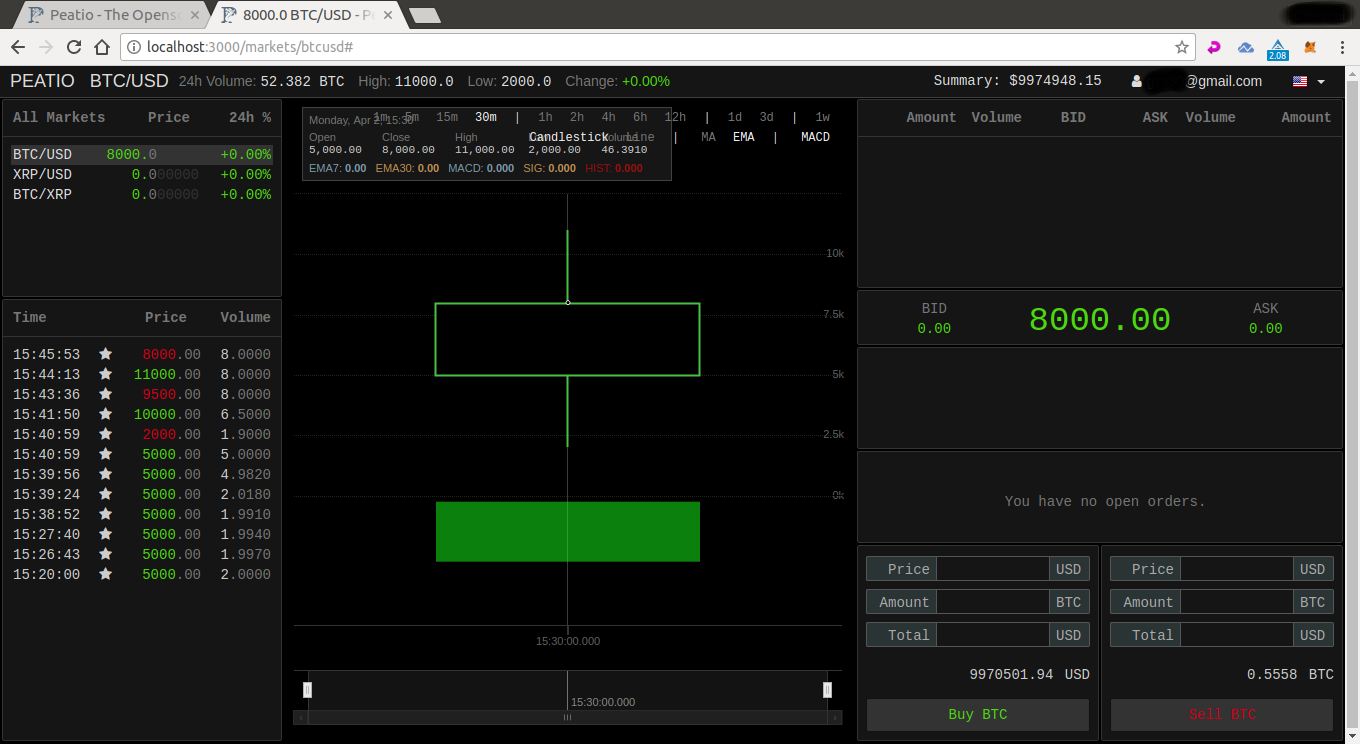
\includegraphics[width=\textwidth*2/3,height=\textheight,keepaspectratio]{RE_TradingUIC}
	\captionof{figure}{UI di trading di Ripa Exchange}
	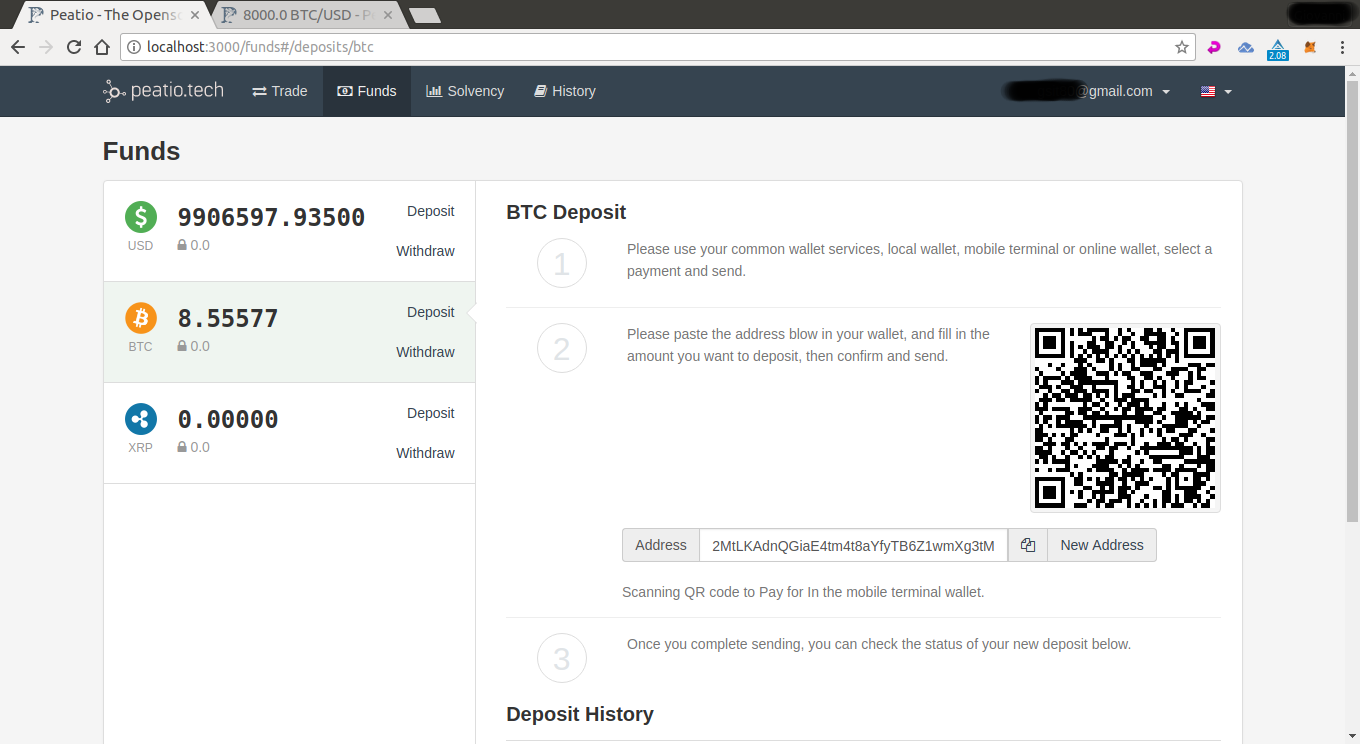
\includegraphics[width=\textwidth*2/3,height=\textheight,keepaspectratio]{RE_depositBTCC}
	\captionof{figure}{UI di deposio/prelievo}
	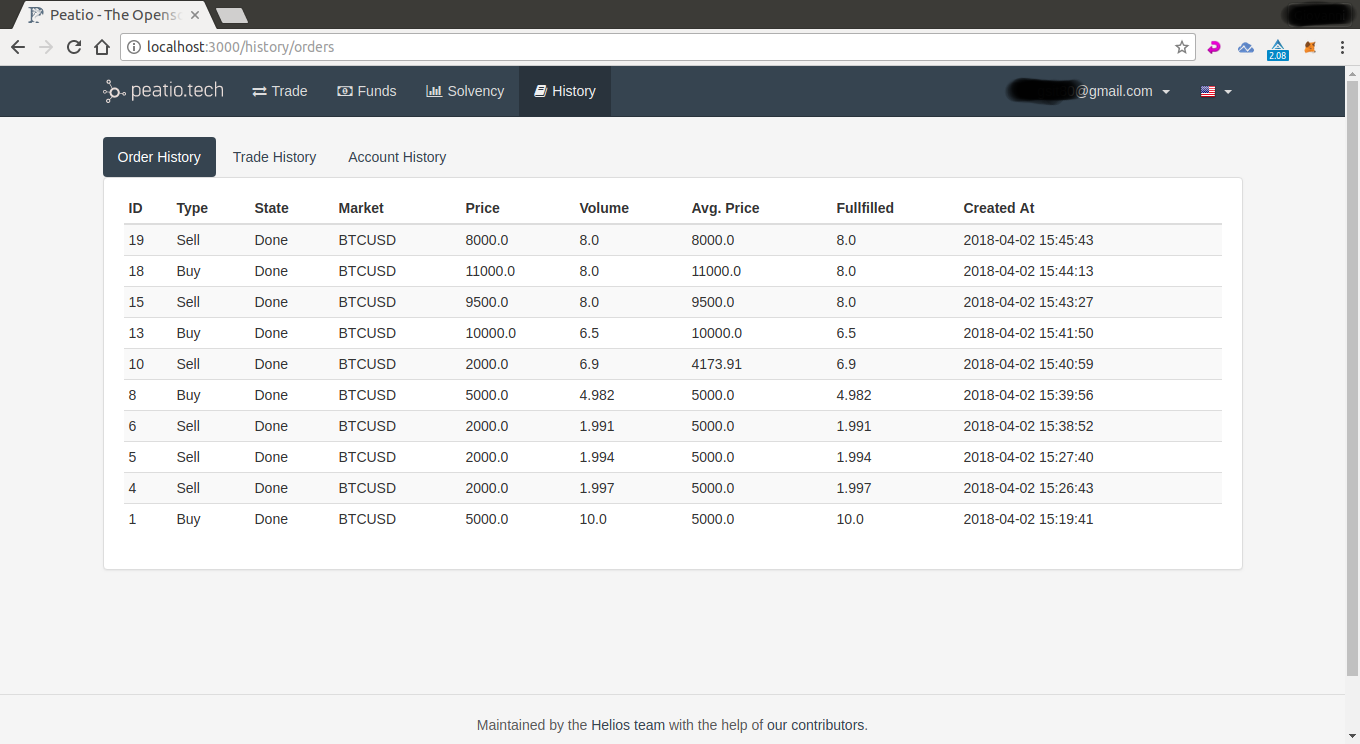
\includegraphics[width=\textwidth*2/3,height=\textheight,keepaspectratio]{RE_historyC}
	\captionof{figure}{UI di storico ordini}
	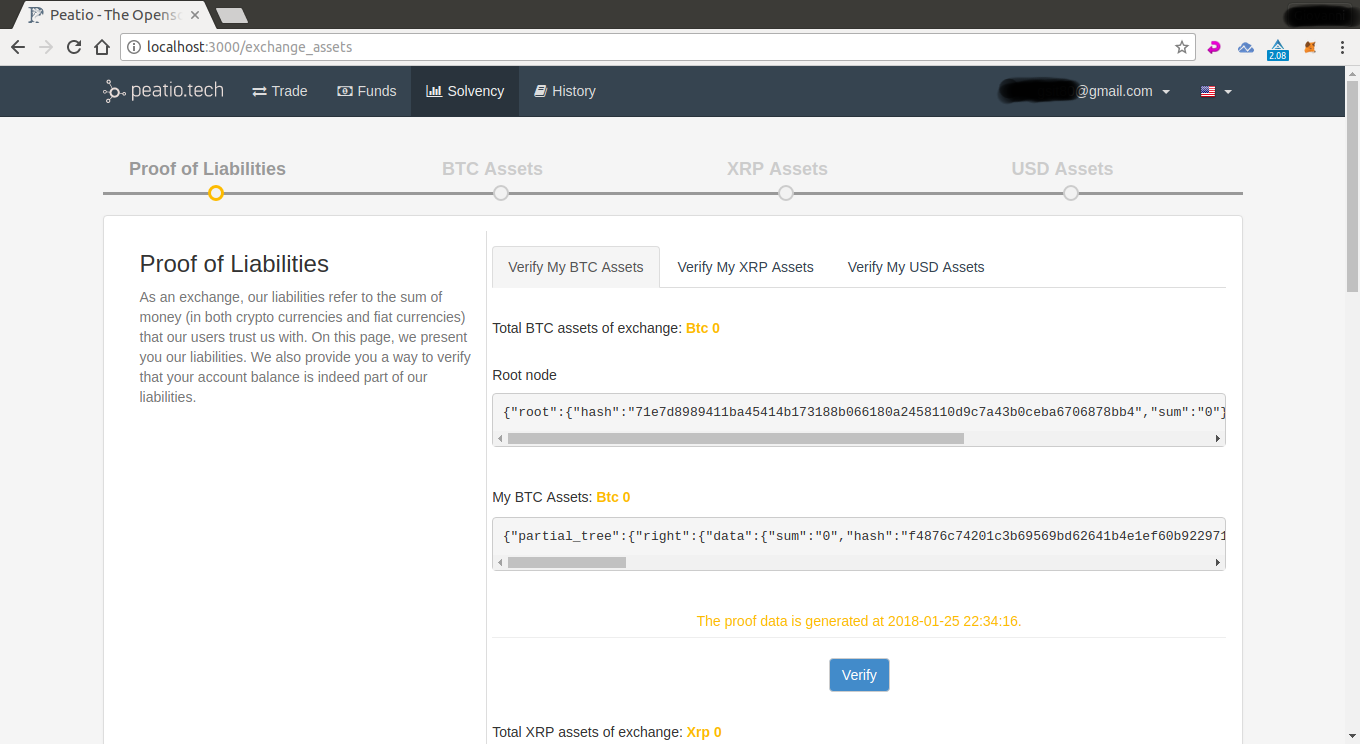
\includegraphics[width=\textwidth*2/3,height=\textheight,keepaspectratio]{RE_solvencyC}
	\captionof{figure}{UI di prova di solvibilità}
\end{center}

\subsection{Admin Interface}
Di seguito alcuni screenshot dell'interfaccia utente dell'area amministrativa dell'exchange Ripa:
\textcolor{darkred}{questi screenshot sono un lavoro in corso e non è detto che rappresentino l'interfaccia utente del prodotto finale}
\begin{center}
	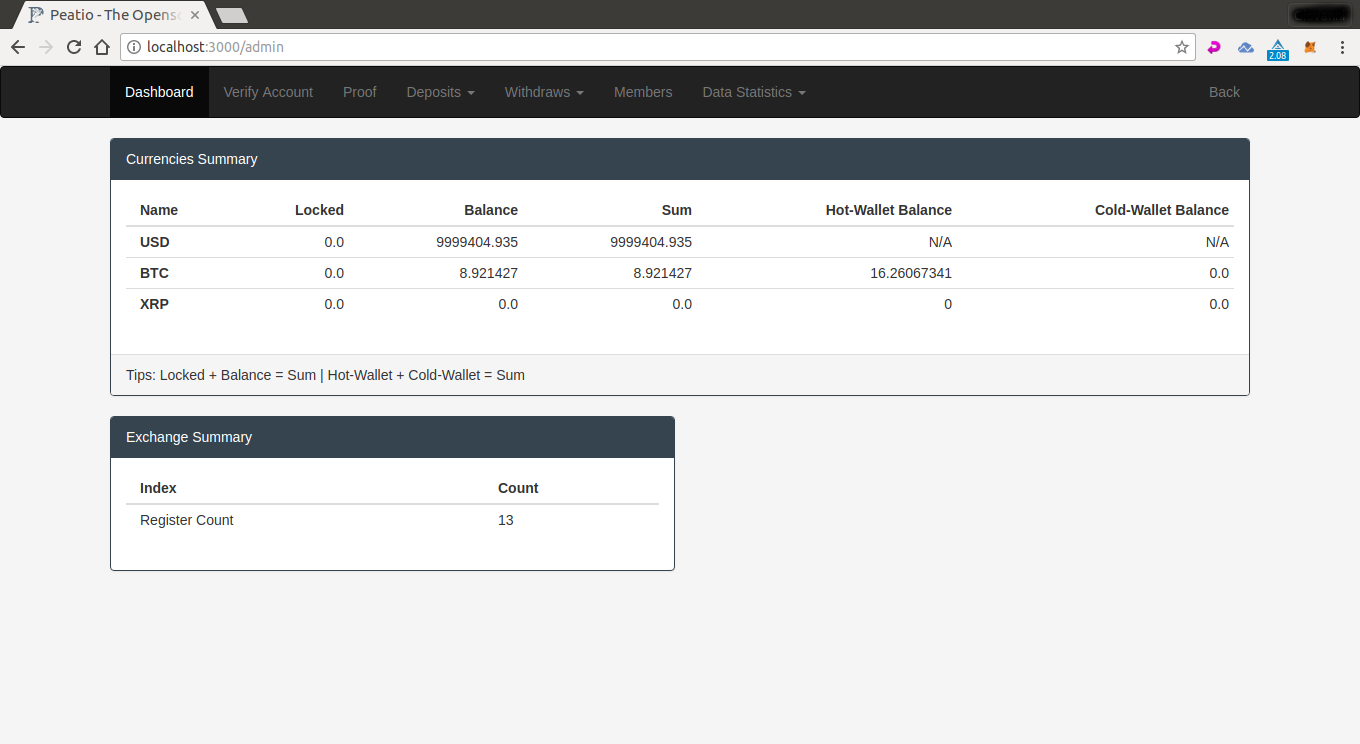
\includegraphics[width=\textwidth*2/3,height=\textheight,keepaspectratio]{RE_adminDashboardC}
	\captionof{figure}{Admin console dashboard}
	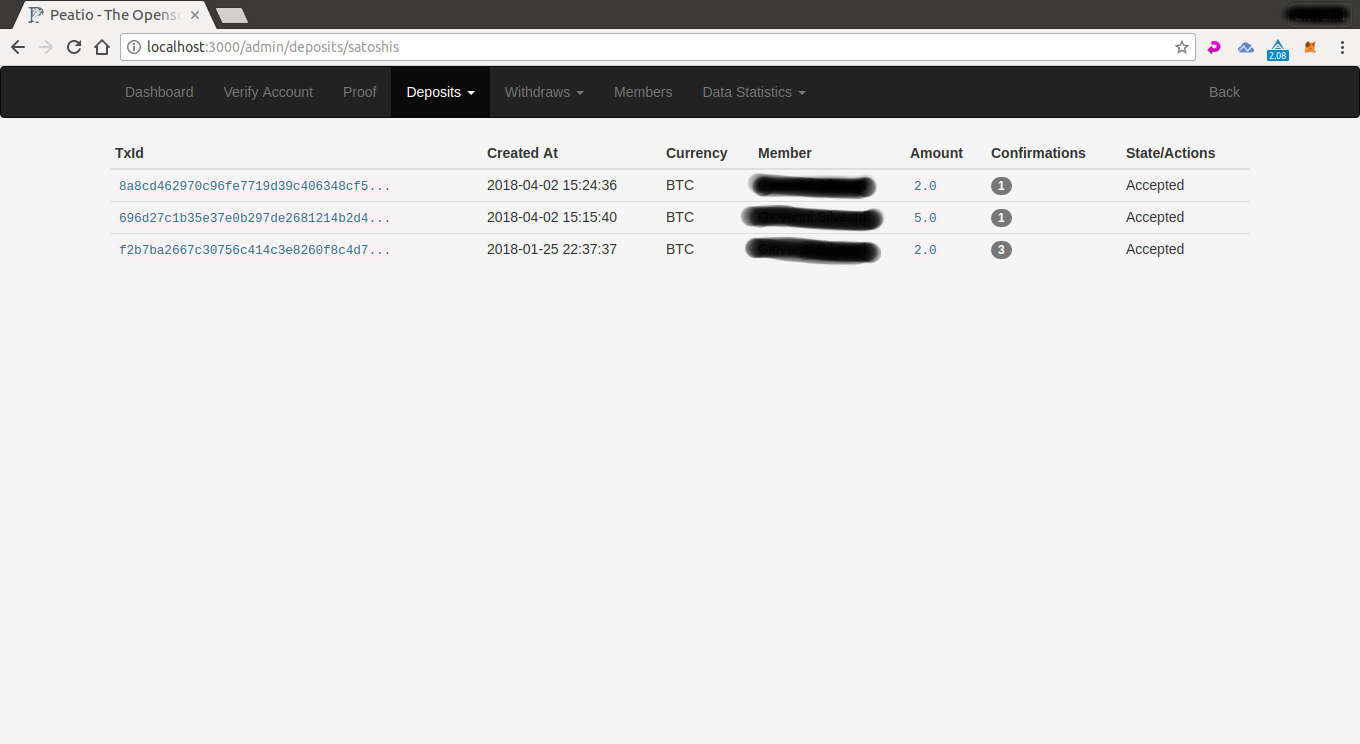
\includegraphics[width=\textwidth*2/3,height=\textheight,keepaspectratio]{RE_adminDepositsC}
	\captionof{figure}{Admin console sezione di deposito}
	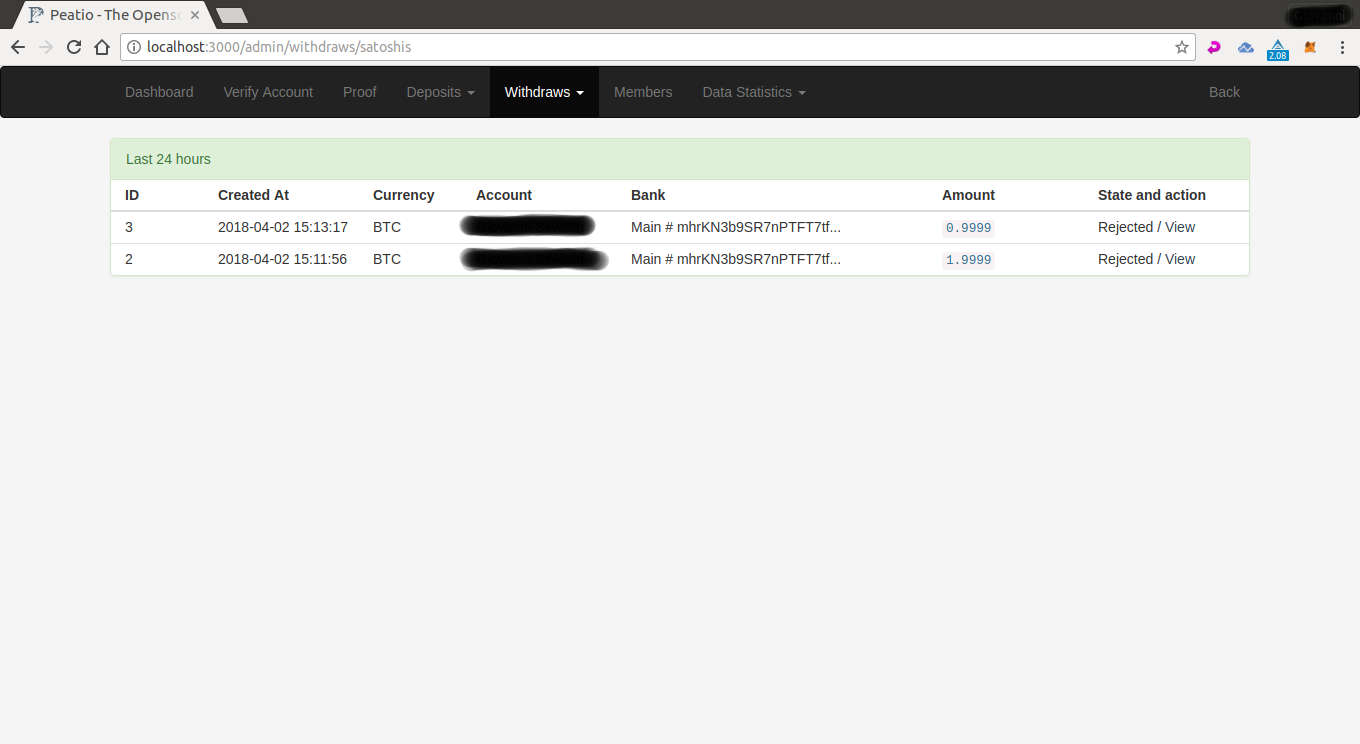
\includegraphics[width=\textwidth*2/3,height=\textheight,keepaspectratio]{RE_adminWithdrawsC}
	\captionof{figure}{Admin console sezione di prelievo}
	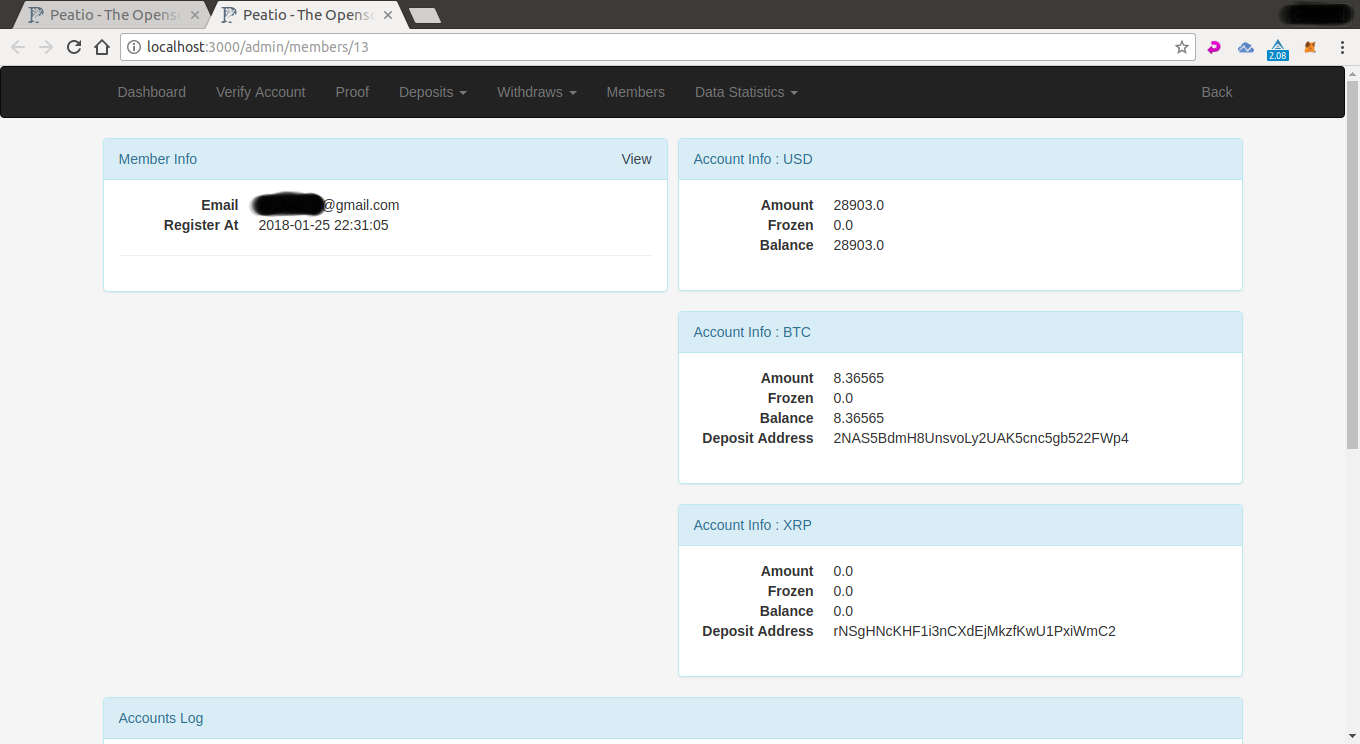
\includegraphics[width=\textwidth*2/3,height=\textheight,keepaspectratio]{RE_adminUserInfo1C}
	\captionof{figure}{Sezione informazioni utente}
	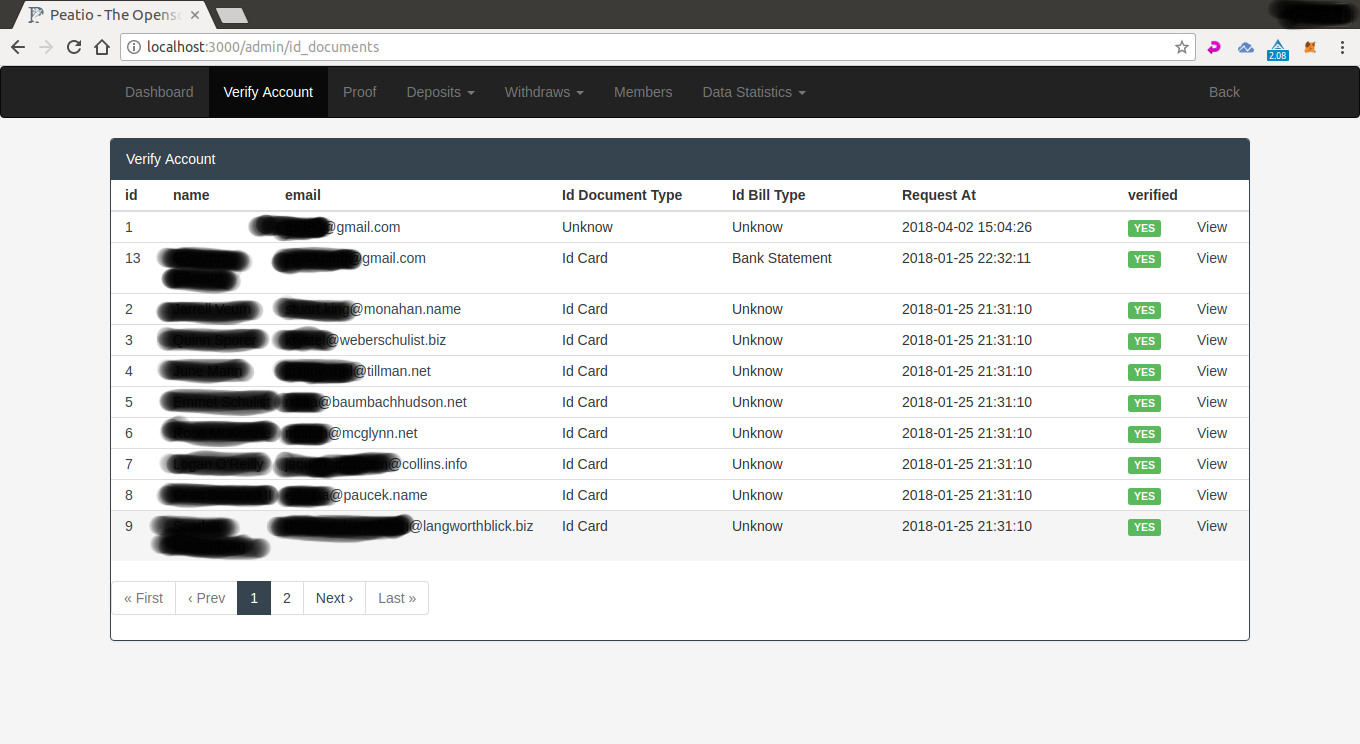
\includegraphics[width=\textwidth*2/3,height=\textheight,keepaspectratio]{RE_adminVerifyAccountC}
	\captionof{figure}{Sezione verifica utente}
\end{center}

\section{Funzionalità al Lancio}
All'apertura della prima istanza di Ripa Exchange le seguenti funzionalità sono previste:
\begin{itemize}
	\item \textsc{\textsc{CRYPTO $\Leftrightarrow$ CRYPTO}}: exchange di cambio valuta virtuale in valuta virtuale
	\item \textsc{\textsc{OAuth}}: Facebook, Google, Twitter
	\item \textsc{\textsc{FIDO}}: login con standard FIDO Alliance
	\item \textsc{\textsc{Protocolli}}: POW, DPOS, Masternode, tether, ERC20 accettati dall'exchange
	\item \textsc{\textsc{Valute}}: BTC, ETH, DOGE, BCH, TUSD, ARK, LISK, SHIFT, RISE, KAPU, OXY, RIPA, token ERC20 promettenti, 
	ed altre valute nella sezione protocolli non citate qui
	\item \textsc{\textsc{Mercati Principali}}: BTC, ETH, ARK
	\item \textsc{\textsc{Tipo di Ordini}}: market, limit
\end{itemize}

\subsection{Funzionalità Future}
Le future istanze di Ripa Exchange implementeranno le seguenti funzionalità:
\begin{itemize}
	\item \textsc{\textsc{E-Wallets}}: OKPay, NETELLER, MoneyPolo, others...
	\item \textsc{\textsc{Funzionalità di Trading Avanzate}}: margin trading, stop loss and take profit, 
	\item \textsc{\textsc{FIAT $\Leftrightarrow$ CRYPTO}}: depositi/prelievi tramite bonifico bancario
	\item \textsc{\textsc{Altre funzionalità}}: VISA/MasterCard, merchants tools, P2P Lending 
\end{itemize}

\section{Verso un Exchange Decentralizzato...}
Ripa Exchange è un exchange centralizzato che sarà convertito in un ibrido-decentralizzato per creare una rete di exchange
che condividono lo stesso codice sorgente e la stessa liquidità in modo tale che tu possa offrire liquitià ai tuoi clienti 
già dal giorno 1 di apertura degli scambi finanziari.\\

Per offrire i PRO di un exchange centralizzato come supporto di livello platino e scambio FIAT, ed i PRO di un exchange 
decentralizzato come la liquidità, senza i CONTRO di entrambi, dovremo eseguire questa passaggio con lo step intermedio di un exchange 
ibrido-decentralizzato e durante la fase 3 del progetto RipaEx (WP 4-6) esguiremo tutte le analisi funzionali e tecniche 
richieste per costruire il prossimo passo su fondamenta solide ed offrire alla comunità RipaEx un exchange open source, sicuro
ed efficiente.

%----------------------------------------------------------------------------------------
%	PART
%----------------------------------------------------------------------------------------

%\part{Part Two}

%----------------------------------------------------------------------------------------
%	CHAPTER 4: Ripa Blockchain
%----------------------------------------------------------------------------------------

\chapterimage{chapter_head_4_Dubai.jpg} % Chapter heading image
\chapter{La Blockchain Ripa}
\label{sec:theRipaBlockchain}
Il progetto RipaEx avrà la propria blockchain che sarà denominata Ripa, securizzata tramite il protocollo DPOS e
con il proprio token XPX (simbolo \PHP) scambiato su di essa che servirà a svolgere le seguenti funzioni:
	\begin{enumerate}
		\item per listare nuove valute nell'exchange
		\item per pubblicizzare nuovi progetti
		\item per comprare gadget RipaEx nello Store RipaEx Store
		\item per pagare per l'acquisto di beni e servizi in rivenditori autorizzati tramite il RipaEx POV (Punto di Vendita)
		\item per condividere liquidità tra tutti gli exchnage della rete Ripa
	\end{enumerate}

Il token XPX è una criptovaluta derivata da ARK, Lisk, Crypti e BitShares con differenze uniche e miglioramenti per 
raggiungere l'obbiettivo di condividere liquidità tra tutti gli exchange della rete Ripa. Tuttavia questo codice eredita
le transazioni semplificate tra le blockchain basate su ARK ed il protocollo di consenso DPOS. Questo codice sorgente omogeneo 
permette lo sviluppo di potenziali servizi inter-blockchain nella forma di app ARK ed assieme ad altri sistemi addizionali
forniti dagli amministratori delle blockchain rispettive.

\vspace{5mm}
\textsc{\textbf{La blockchain Ripa è un fork di ARK e la creazione di tale blockchain serve per completare l'ecosistema Ripa
permettendo ogni exchange nella rete Ripa di condividere la stessa liquidità. Noi ci affideremo sempre ad ARK come nostro
fornitore di tecnologia blockchain di fiducia per includere il loro codice nei nostri repositori
per tutto ciò che riguarda la blockchain Ripa}}

\vspace{5mm}

Spiegato l'uso della blockchain Ripa all'interno dell'ecosistema RipaEx e spiegato il legame di partnership tecnologica
RIPA - ARK nelle seguenti sezioni potete trovare le specifiche della blokchain Ripa che sono derivata da ARK ed alcune sviluppate 
``ad hoc'' per l'ecosistema Ripa.

\section{Tecnologia Delegated Proof of Stake}
Ripa Blockchain eredita il sistema di consenso Delegated Proof of Stake (DPoS) che è stato inizialmente
introdotto da BitShares. Questo algoritmo di consenso è stato progettato per eliminare i problemi dell'algoritmo
Proof of Work (PoW), nello specifico la centralizzazione del potere computazionale e l'esponenziale uso di energia
elettrica. Anche se non completamente decentralizzato in quanto si basa su di un numero fisso di delegati eletti
dalla comunità, il DPoS garantisce migliore decentralizzazione di Bitcoin. L'algoritmo di consenso è migliorato
con il tempo, evolvendo in una procedura di consenso ottimale con il tempo.\\

Le specifiche tecniche di Ripa Blockchain sono le seguenti:
\begin{enumerate}
	\item DPoS (Delegated Proof of Stake)
	\begin{itemize}
		\item 101 delegati forgiani
		\item Delegati selezionati mediate un meccanismo di voto insito nel sistema DPoS
		\item 115,000,000 XPX - Forgiati nel Genesis Block
	\end{itemize}
	\item Account Multi-firma
	\item Reward di Blocco Costante
	\begin{itemize}
		\item 2 \PHP per blocco
		\item Livello di Inflazione (con blocco da 8s)
		\begin{itemize}
			\item 6.31\% per il primo anno
			\item 5.93\% il secondo anno
			\item 4.02\% il decimo anno
		\end{itemize}
		\item Tempo di forgiatura blocco di 8 secondi
		\begin{itemize}
			\item Tempo di forgiatura blocco riducibile nel tempo con aggiornamenti futuri del core.
		\end{itemize}
		\item 25 transazioni per blocco
		\begin{itemize}
			\item Incrementabile con soft fork se richiesto.
		\end{itemize}
	\end{itemize}
	\item Tabelle di routing
	\item Campo SmartBridge per uso con blockchain connesse alla blockchain RIPA principale (ARK Contract Execution Service)
	\item Transazioni batch\footnote{Aggiornamento futuro: quando ARK 2.0 sarà rilasciata \label{note1}}
	\item Fee di transazione personalizzabili\footnotemark[\value{footnote}]
	\item SmartContract nativi\footnote{Aggiornamento futuro: quando ARK Virtual Machine sarà rilasciata}
\end{enumerate}

\vspace{5mm}
\textsc{\textbf{Come detto Ripa Blockchain è un fork di ARK e noi ci affideremo sempre ad ARK come nostro provider di tecnologia 
di fiducia per includere il loro codice nelle nostre ultime funzionalità per tutto ciò che concerne lo sviluppo di 
Ripa Blockchain}}, funzionalità quali:
\begin{itemize}
	\item \textbf{Scalabilità della rete} al livello delle reti di Carte di Credito più diffuse con aggiornamento del core
	\begin{itemize}
		\item Aumentare il numero dei delegati forgianti
		\item Aumentare le dimensioni del blocco per includere più transazioni
		\item Implementazione del concetto di blocchi pre-approvati PBFT in testnet [nome in codice: TwinChain]
		\item Tabelle di routing per minimizzare i salti tra i nodi quando i blocchi sono trasmessi
		\item Inclusione di forgiato con nipoti RIPA
	\end{itemize}
	\item \textbf{Due tipi di nodi} sono usati per sicurizzare la rete RIPA:
	\begin{itemize}
		\item \textbf{Nodi di trasmissione} - Nodi con funzionalità di API che servono come back-end per servizi terzi
		(es: lite client). I nodi di trasmissione non forgiano blocchi e non quadagnano XPX per le transazioni.
		\item \textbf{Nodi forgianti} - Nodi con funzionalità API ridotta per abbassare l'esposizione a potenziali
		attacchi DDoS alla piattaforma RIPA. I nodi forgianti forgiano XPX e ricevono commissioni di transazione.
	\end{itemize}
	\item \textbf{Lite client ufficiale} per l'accesso al network è forinito poco dopo il lancio della mainnet ed 
	include il client desktop (Windows, MacOS e Linux) ed il client mobile (Android ed iOS)
	\item \textbf{Creazione offline di indirizzi}: la rete di per se non ha una Interfaccia Grafica Utente di 
	default, ogni account RIPA può essere creato off-line e gestito a costo zero su di un singolo dispositivo
	(computer, smartphone, tablet, ARM, IoT).
\end{itemize}

\section{Hierarchical Deterministic (HD) Wallets (BIP32)}
La struttura della chiave pubblica e privata di RIPA segue le stesse specifiche di Bitcoin. Una implementazione
personalizzata del protocollo BIP32 per Wallet Hierarchical Deterministic è fornita agli utenti RIPA.

\section{Commissioni}
Le commissioni per una transazione standard sono \PHP0,10 ma saranno flessibili in futuri rilasci di Ripa Blockchain.
Al lancio della mainnet, la struttura delle commissioni è fornita preconfigurata e pronta all'uso ai delegati
forgianti secondo le seguenti regole:
	\begin{itemize}
		\item Transazione \PHP0.1
		\item Voto \PHP1 (101 voti per transazione)
		\item Seconda Firma \PHP1
		\item Multi Firma \PHP1 per firma + \PHP1 per account firmatario
		\item Registrazione di un delegato \PHP25.
	\end{itemize}
Tutte le commissioni sono pagate ai nodi forgianti che processano i blocchi contenenti quelle commissioni.

\section{Delegati Ripa e Votazione}
Ogni nodo che esegue il codice della blockchain Ripa che vuole forgiare blocchi deve registrarsi come 
delegato pagando la commissione di 25 \PHP. Ripa incorpora un nuovo sistema di voto DPoS
originariamente progettato dai fondatori di Crypti. La commissione di voto è di 1 \PHP, 
il peso di voto di ciascun wallet è suddiviso equamente tra tutti i delegati votati 
nella transazione. Ad esempio: 
\begin{itemize}
	\item Se un wallet vota per un delegato, il delegato riceve il 100\% del peso di voto del
	wallet.
	\item Se il wallet vota per un delegato addizionale, il peso di voto totale è 
	suddiviso equamente tra entrambi i delegati al 50\%.
	\item Aggiungendo un terzo delegato, il peso di voto è suddiviso nuovamente, 
	ed ogniuno dei tre delegati riceve il 33,333\% del peso di voto del wallet.
\end{itemize}

I 101 delegati forgianti con il numero di voti maggiore sono elegibili per forgiare blocchi
RIPA. Questa progettazione elimina la possibilità che un singolo grande possessore di
RIPA oppure un'organizzazione che detiene una larga percentuale di RIPA siano in grado
di prendere il controllo della rete nella sua interezza mediante il voto dei loro nodi
ponendoli in posizione di nodi forgianti, prendendo, effettivamente controllo dell'intera rete. 
I voti provenienti dai token RIPA in possesso del Ripa Founder Team
possono essere usati a sola discrezione del team Ripa.

\section{Collegamenti tra Blockchain}
\subsection{Blockchain Connesse ARK (Tecnologia SmartBridge)}
La piattaforma ARK 1.0 non fornisce supporto diretto per sidechain o dapp. Invece
un meccanismo per connettere direttamente blockchain tra loro e con la blockchain ARK
è fornito tramite una funzione ponte codificata direttamente nel core ARK in cui
ogni blockchain può inviare e ricevere funzioni attivabili a comando e dati
informativi passando per la rete ARK principale tramite \textbf{Endoded Listeners}
e \textbf{SmartBridge} appositamente sviluppati.
\begin{center}
	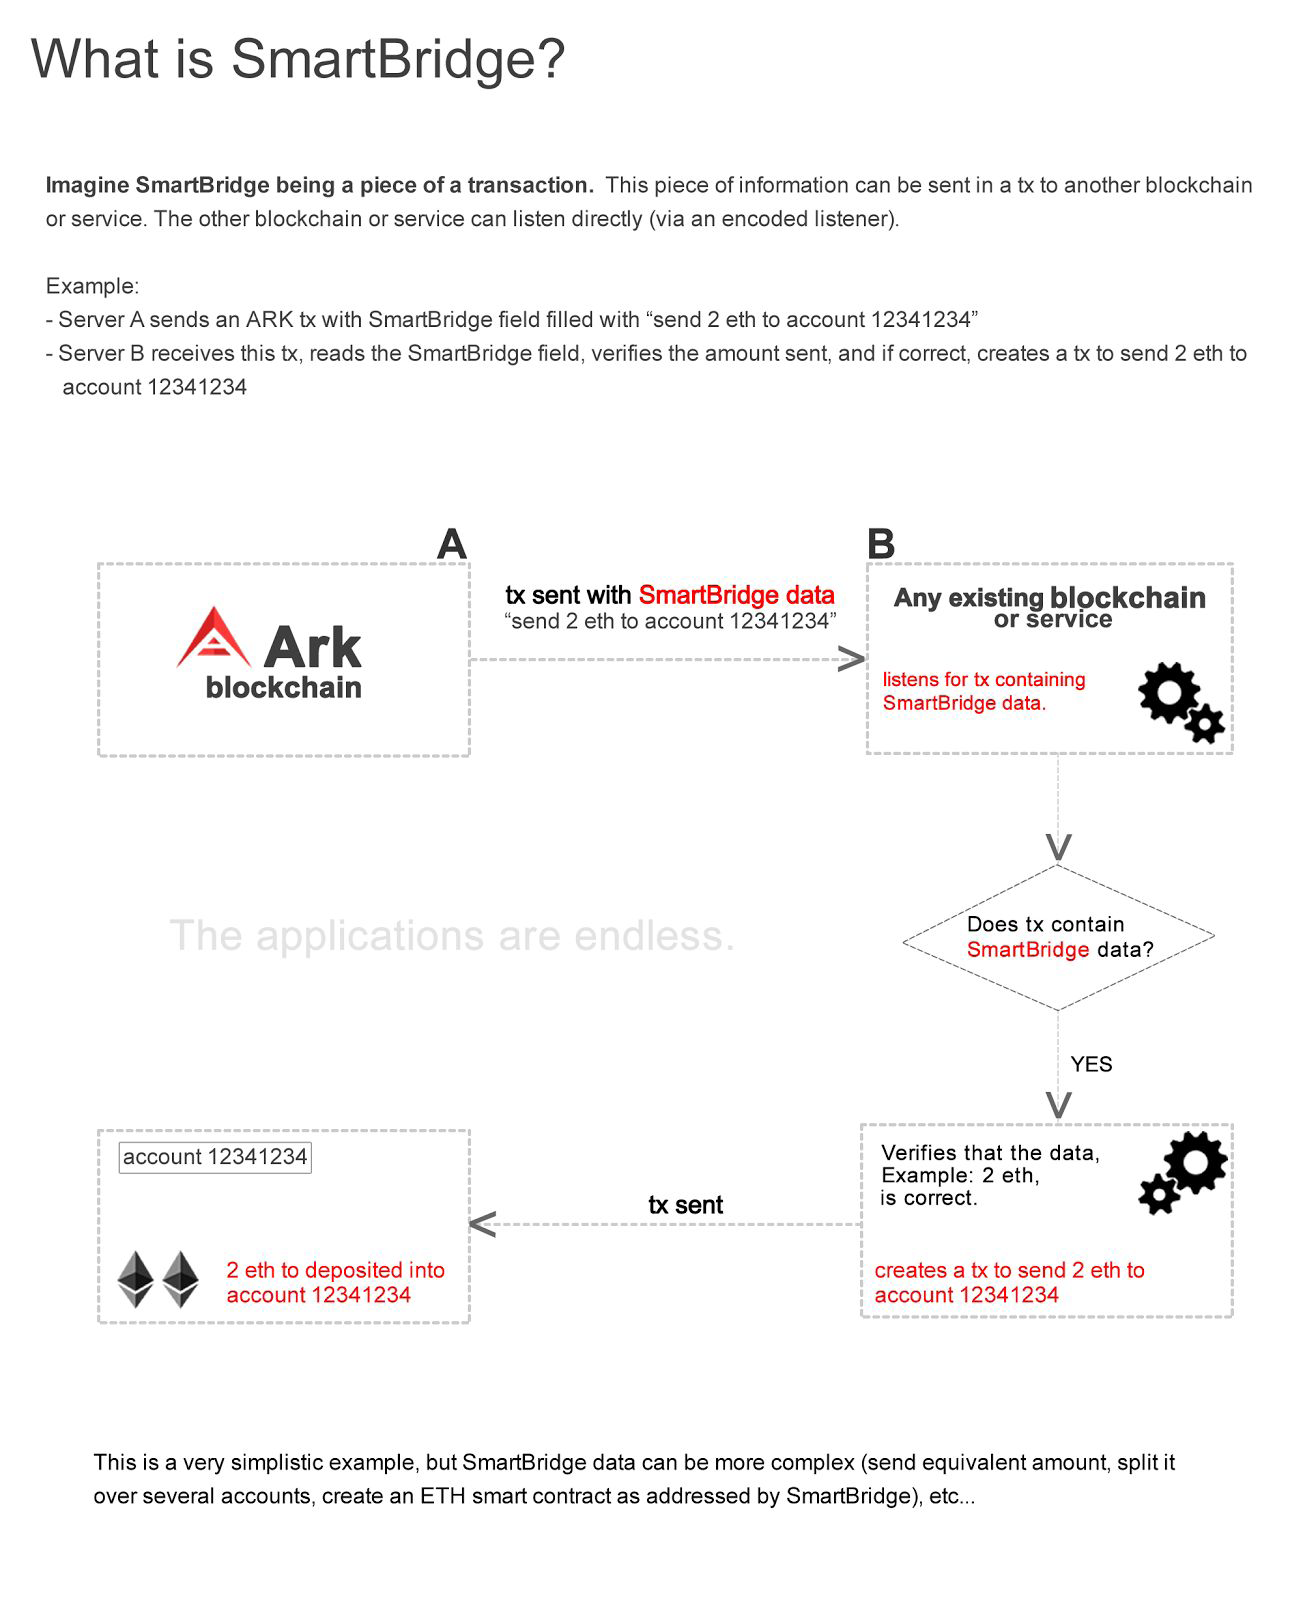
\includegraphics[width=\textwidth,height=\textheight,keepaspectratio]{ARKSmartBridge}
	\captionof{figure}{ARK Tecnologia SmartBridge}
\end{center}

\subsection{A.C.E.S. - ARK Contract Execution Service}
ACES è una piattaforma di interoperabilità tra blockchain che fornisce protocolli semplificati
e strumenti per costruire mercati di scambio servizi tra blockchain robusti.

ACES è composta principalmente dai tre componenti seguenti:
\begin{itemize}
	\item \textbf{Listener} i Listener ACES forniscono una via per tutti gli eventi delle diverse
	blockchain per essere facilmente consumanti via servizi REST. Le API permettono agli utenti
	di creare sottoscrizioni e ricevere eventi blockchain in tempo-reale usando callback Webhook.
	\item \textbf{Servizi} ACES che creano ed eseguono Service Contract, che possono essere qualsiasi
	cosa da caricare un file in una blockchain di dati, ad eseguire trasmissione di valore,
	creare smart contract, eseguire codice su di una piattaforma di computer distribuita, oppure
	interagire con dispositivi IoT.
	\item \textbf{Console di Mercato} di ACES è una dashboard utente per cercare ed eseguire Service
	Contract listati nel marketplace. I provider ACES possono listare i servizi dei loro nodi 
	usando le API del marketplace.
\end{itemize}

\begin{center}
	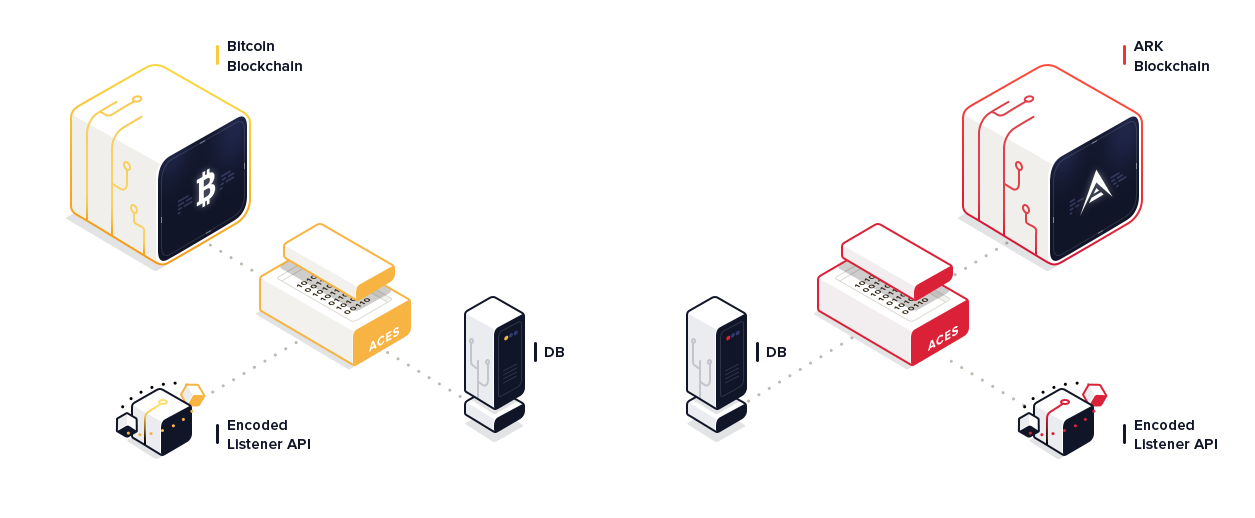
\includegraphics[width=\textwidth,height=\textheight,keepaspectratio]{ACES}
	\captionof{figure}{Implementazione SmartBridge ARK-BTC di A.C.E.S.}
\end{center}

\section{Ripa Liquidity Service Provider (R.L.S.P)}
Usando la tecnologia SmartBridge RipaEx svilupperà un meccanismo per condividere liquidità tra tutti gli exchange della rete
Ripa scrivendo i singoli orderbook in Ripa Blockchain ed eseguendo accoppiamento di ordini tra tutti gli exchange della rete.

In questo modo puoi avere i benefici di un exchange decentralizzato (come ad esempio la liquidità) con i benefici di un 
exchange centralizzato (come ad esempio customer support di livello platino e scambio FIAT).

\section{Ripa Community Fund}
Per permettere la nascita di nuovi exchange nella rete Ripa viene creato all'avvio del progetto il Fondo Comunitario Ripa - RCF - 
con le seguenti caratteristiche:
\begin{itemize}
	\item \textbf{Fondi di Partenza}: l'RCF avrà un capitale iniziale operativo pari al 5\% (5.750.000 \PHP) del blocco genesis
	\item \textbf{Fondi Ricorrenti}: ogni delegato contribuirà all'RCF con il 5\% degli XPX forgiati settimanalmente
\end{itemize}
\vspace{5mm}
Per ottenere i fondi dell'RCF per avviare il tuo Ripa Exchange devi inoltrare il tuo proposal nel sito ufficiale dell'RCF oppure
nella sezione RCF del forum Ripa in qualsiasi momento dopo l'avvio della prima istanza funzionante di Ripa Exchange.

%----------------------------------------------------------------------------------------
%	CHAPTER 5: Token Sale
%----------------------------------------------------------------------------------------

\chapterimage{chapter_head_5_Tokyo.jpg} % Chapter heading image
\chapter{Vendita Token}
\section{Introduzione}
La vendita di token RipaEx XPX sarà separata in due fasi:
	\begin{itemize}
		\item \textbf{\textsc{PreSale}}: che durerà da Aprile a Giugno 2018
		\item \textbf{\textsc{RIPA TEC}}: che durerà da Luglio a Dicembre 2018
	\end{itemize}
\vspace{5mm}
Colloquialmente le fasi di PreSale e RIPA TEC possono essere identificate con l'appellativo \textit{RipaEx ICO}.

\subsection{Tasso di Cambio e Criptomonete Accettate}
Durante la vendita dei token il tasso di cambio per i token XPX sarà di \textbf{\PHP/\euro0,10}.\\

Le seguenti valute virtuali sono accettate: \textbf{BTC, ETH, ARK, LISK}.\\

Se volete inviarci criptomonete diverse da queste inoltrateci la vostra scelta e vi indicheremo immediatamente
se possiamo eseguire lo scambio ed i dettagli di come eseguirlo (indirizzo di recezione, tasso di cambio,
quantità)\\

\textsc{Il tasso di cambio è Bitstamp last ed è valido per 60 minuti dopo la ricezione del preventivo}.

\subsection{Bonus per gli Investitori e per i nuovi Iscritti}
A tutti gli investitori del progetto RipaEx sarà concesso un credito di \euro1.000,00 sulle commissioni
di transazione al lancio della prima istanza di Ripa Exchange, mentre verrà consegnato un bonus di \PHP1.000,00
a tutti i nuovi iscritti nell'exchange da utilizzare come si vuole.

\section{Come Investire}
\subsection{PreSale di Token Ripa XPX}
La vendita privata dei token XPX è \textbf{cominciata Lunedi 02/04/2018 alle 00:00 GMT e finirà Domenica
01/07/2018 alle 23:59 GMT}.

I token XPX possono essere comprati direttamente al seguente link:
\begin{center}
	\href{https://www.ripaex.io/privsale}{\textsc{www.ripaex.io/privsale}}
\end{center}

oppure inviate le vostre richieste di acquisto in
\href{https://join.slack.com/t/ripaex/shared_invite/enQtMzM4NzUwNjU4OTQ0LTY3MDJmMTdhYTNlZjJlNGUxNzM1YjUwYjgyYjZlMDJmOTg3NTIzNThmNTYyMGQ3ODBkOTRmYzk3Y2Y4MzBkOTY}{Slack}, 
\href{https://t.me/ripaex}{Telegram}, Facebook, Twitter oppure altri social media in cui siamo presenti
i cui link sono presenti nella Sezione \ref{sec:social}.
Per tutta la durata del periodo di vendita privata ogni operazione di scambio \textbf{sarà eseguita al tasso di cambio di
\PHP/\euro0,0500 fino a che i primi 5.000.000 di token XPX} non sono stati venduti ed al tasso di cambio di \PHP/\euro0,05714286 dopo di allora.

\subsection{RIPA TEC}
La raccolta fondi tramite la piattaforma RIPA TEC seguirà il seguente programma:
\begin{itemize}
	\item \textcolor{airforceblue}{\textbf{\textit{Exchange} da 02/07/2018 a 15/07/2018}}: al tasso di \PHP/\euro0,0500 (\textcolor{airforceblue}{\textbf{100\% bonus}})
	\item \textcolor{darkgoldenrod}{\textbf{\textit{Cooling-OFF} da 16/07/2018 a 22/07/2018}}: 
	al tasso di \PHP/\euro0,05128205 (\textcolor{darkgoldenrod}{\textbf{95\% bonus}})
	\item \textcolor{airforceblue}{\textbf{\textit{Exchange} da 23/07/2018 a 05/08/2018}}: al tasso di \PHP/\euro0,05714286 (\textcolor{airforceblue}{\textbf{75\% bonus}})
	\item \textcolor{darkgoldenrod}{\textbf{\textit{Cooling-OFF} da 06/08/2018 a 12/08/2018}}: 
	al tasso di \PHP/\euro0,05847953 (\textcolor{darkgoldenrod}{\textbf{74\% bonus}})
	\item \textcolor{airforceblue}{\textbf{\textit{Exchange} da 13/08/2018 a 26/08/2018}}: al tasso di \PHP/\euro0,06666667 (\textcolor{airforceblue}{\textbf{50\% bonus}})
	\item \textcolor{darkgoldenrod}{\textbf{\textit{Cooling-OFF} da 27/08/2018 a 02/09/2018}}: 
	al tasso di \PHP/\euro0,06802721 (\textcolor{darkgoldenrod}{\textbf{47\% bonus}})
	\item \textcolor{airforceblue}{\textbf{\textit{Exchange} da 03/09/2018 a 16/09/2018}}: al tasso di \PHP/\euro0,07142857 (\textcolor{airforceblue}{\textbf{40\% bonus}})
	\item \textcolor{darkgoldenrod}{\textbf{\textit{Cooling-OFF} da 17/09/2018 a 23/09/2018}}: 
	al tasso di \PHP/\euro0,07246377 (\textcolor{darkgoldenrod}{\textbf{38\% bonus}})
	\item \textcolor{airforceblue}{\textbf{\textit{Exchange} da 24/09/2018 a 07/10/2018}}: al tasso di \PHP/\euro0,07692308 (\textcolor{airforceblue}{\textbf{30\% bonus}})
	\item \textcolor{darkgoldenrod}{\textbf{\textit{Cooling-OFF} da 08/10/2018 a 14/10/2018}}: 
	al tasso di \PHP/\euro0,07751938 (\textcolor{darkgoldenrod}{\textbf{29\% bonus}})
	\item \textcolor{airforceblue}{\textbf{\textit{Exchange} da 15/10/2018 a 28/10/2018}}: al tasso di \PHP/\euro0,08333333 (\textcolor{airforceblue}{\textbf{20\% bonus}})
	\item \textcolor{darkgoldenrod}{\textbf{\textit{Cooling-OFF} da 29/10/2018 a 04/11/2018}}: 
	al tasso di \PHP/\euro0,08403361 (\textcolor{darkgoldenrod}{\textbf{19\% bonus}})
	\item \textcolor{airforceblue}{\textbf{\textit{Exchange} da 05/11/2018 a 18/11/2018}}: al tasso di \PHP/\euro0,09090909 (\textcolor{airforceblue}{\textbf{10\% bonus}})
	\item \textcolor{darkgoldenrod}{\textbf{\textit{Cooling-OFF} da 19/11/2018 a 25/11/2018}}: 
	al tasso di \PHP/\euro0,09174312 (\textcolor{darkgoldenrod}{\textbf{9\% bonus}})
	\item \textcolor{airforceblue}{\textbf{\textit{Exchange} da 26/11/2018 a 09/12/2018}}: al tasso di \PHP/\euro0,0952381 (\textcolor{airforceblue}{\textbf{5\% bonus}})
	\item \textcolor{darkgoldenrod}{\textbf{\textit{Cooling-OFF} da 09/12/2018 a 16/12/2018}}: 
	al tasso di \PHP/\euro0,09615385 (\textcolor{darkgoldenrod}{\textbf{4\% bonus}})
\end{itemize}
\vspace{5mm}
La distribuzione dei token avverrà alla fine di ogni giorno lavorativo ed eseguita automaticamente
tramite la piattaforma RIPA TEC. Il target minimo da raggiungere sono 25 BTC.\\

\textsc{Dal momento che il tasso di cambio del token XPX è calcolato nei rispetti della divisa euro tu, come investitore,
hai la garanzia che non perderai nessun fondo investito durante il periodo di vendita token in quanto i token XPX
saranno listati nei nostri exchange agli inizi del 2019 allo stesso tasso di cambio \textbf{\PHP/\euro0,10} 
concordato durante le fasi di PreSale e RIPA TEC}.\\

La piattaforma RIPA TEC sarà disponibile al seguente link dopo Luglio 2018:
\begin{center}
	\href{https://tec.ripaex.io}{\textsc{tec.ripaex.io}}
\end{center}
seguici in Facebook, Twitter, 
\href{https://t.me/ripaex}{Telegram}, 
\href{https://join.slack.com/t/ripaex/shared_invite/enQtMzM4NzUwNjU4OTQ0LTY3MDJmMTdhYTNlZjJlNGUxNzM1YjUwYjgyYjZlMDJmOTg3NTIzNThmNTYyMGQ3ODBkOTRmYzk3Y2Y4MzBkOTY}{Slack}
e nei nostri canali social ufficiali per sapere la data esatta di avvio di
RIPA TEC!!

\section{Distribuzione dei Token Ripa XPX}
\textbf{115.000.000} di token XPX sono forgiati nel genesis block: la distribuzione dei token generati è descritta
in figura \ref{fig:distribution} ed in tabella \ref{tab:distribution}.

\vspace{5mm}
%\begin{center}
	\begin{tikzpicture}
		\pie [rotate = 180, explode={0.2, 0.1, 0.1, 0.1, 0.1, 0.1}, radius = 3]
		{65/PreSale e RIPA TEC,
		15/RIPA Founders Team, 
		6/for marketing,
		5/for bounties,
		5/for RCF,
		4/Ark.io SCIC}
	\end{tikzpicture}
	\captionof{figure}{Distribuzione dei token Ripa XPX}	
	\label{fig:distribution}
%\end{center}

\vspace{5mm}
\begin{table}[H]
	\centering
	\begin{tabular}{l l l}
		\toprule
		\textbf{Percentage (\%)} & \textbf{Quantity (\PHP)} & \textbf{Purpose} \\
		\midrule
		65		& 74,750,000	& da distribuire nelle fasi di PreSale e RIPA TEC	\\
		15      & 17,250,000	& da distribuire al RIPA Founders Team	\\
		6       & 6,900,000		& per il marketing	\\
		5       & 5,750,000 	& per i bounties	\\
		5       & 5,750,000		& per il Ripa Community Fund - RCF	\\
		4       & 4,600,000		& per il Ark.io SCIC \\
		\bottomrule
	\end{tabular}
	\captionof{table}{Distribuzione dei token Ripa XPX}
	\label{tab:distribution}
\end{table}

\vspace{5mm}
\textbf{I token non venduti durante le fasi di PreSale e RIPA TEC saranno distrutti} per sempre per permettere
un'equa distribuzione dei fondi raccolti e per evitare speculazioni sui token rimasti.

\section{Divisione dei Fondi}
I fondi raccolti durante le fasi di PreSale e RIPA TEC saranno divisi come indicato in figura \ref{fig:division} 
ed in tabella \ref{tab:division} a seguire

\vspace{5mm}
\begin{tikzpicture}
	\pie [rotate = 180, explode={0.2, 0.1, 0.1}, radius = 3]
	{60/per sviluppo del progetto,
	20/per marketing, 
	20/per supporto legale}
\end{tikzpicture}
\captionof{figure}{Divisione dei fondi}	
\label{fig:division}

\vspace{5mm}
\begin{table}[H]
	\centering
	\begin{tabular}{l l}
		\toprule
		\textbf{Percentage (\%)} & \textbf{Purpose} \\
		\midrule
		60		& per sviluppo del progetto	\\
		20		& per marketing	\\
		20		& per supporto legale	\\
		\bottomrule
	\end{tabular}
	\captionof{table}{Divisione dei fondi}
	\label{tab:division}
\end{table}

\vspace{5mm}
dove la riga di allocazione fondi ``per sviluppo del progetto'' è ulteriormente dettagliata in 
tabella \ref{tab:focus} a seguire.

\vspace{5mm}
\begin{table}[H]
	\centering
	\begin{tabular}{l l}
		\toprule
		\textbf{Percentage (\%)} & \textbf{Purpose} \\
		\midrule
		50		& analisi funzionale, analisi tecnica, sviluppo, collaudo	\\
		20		& supporto tecnico	\\
		15		& infrastruttura	\\
		10		& sicurezza	\\
		5		& analisi di utilizzo	\\
		\bottomrule
	\end{tabular}
	\captionof{table}{Focus per lo sviluppo del progetto}
	\label{tab:focus}
\end{table}

%----------------------------------------------------------------------------------------
%	CHAPTER 6: Economic Projections
%----------------------------------------------------------------------------------------

\chapterimage{chapter_head_6_Frankfurt.jpg} % Chapter heading image

\chapter{Modello di Business}

\section{Obbiettivi del Progetto}
A seguire la matrice di sviluppo per area di interessa basata sulla quantità di fondi raccolti durante le fasi di
PreSale e RIPA TEC:
\begin{tcbraster}[raster columns=5,raster rows=1,raster height=0.8cm,
	valign=center, halign=center,
	enhanced,size=small,sharp corners,colframe=azure(colorwheel),coltext=white,
	colback=azure(colorwheel),fit algorithm=hybrid* ]
	\tcboxfit{}
	\tcboxfit{\textbf{25 BTC}}
	\tcboxfit{\textbf{50 BTC}}
	\tcboxfit{\textbf{250 BTC}}
	\tcboxfit{\textbf{1000 BTC}}
\end{tcbraster}
\begin{tcbraster}[raster columns=5,raster rows=4,raster height=10cm,
	valign=center, halign=center,
	enhanced,size=small,sharp corners,colframe=silver,coltext=black,
	colback=silver,fit algorithm=hybrid* ]
	\tcboxfit{\textsc{\textbf{Sviluppo}}}
	\tcboxfit{\tcbfontsize{0.8} Rilascio exchange CRYPTO $\Leftrightarrow$ CRYPTO con 25 criptovalute supportate 
	e 3 coppie di trading maggiori}
	\tcboxfit{\tcbfontsize{0.8} Rilascio exchange CRYPTO $\Leftrightarrow$ FIAT con carta prepagata MasterCard, 
	50 criptovalute supportate e 3 coppie di trading maggiori}
	\tcboxfit{\tcbfontsize{0.8} Funzionalità di trading avanzato, apertura di un secondo e terzo 
	Ripa Exchange all'interno della rete Ripa}
	\tcboxfit{\tcbfontsize{0.8} Apertura di dieci Ripa Exchange in ogni locazione terrestre}

	\tcboxfit{\textsc{\textbf{Marketing}}}
	\tcboxfit{\tcbfontsize{0.8} Supporto da un'agenzia, campagne pubblicitarie mirate sui canali interessati}
	\tcboxfit{\tcbfontsize{0.8} Supporto da due agenzie, campagne pubblicitarie maggiori, negozio di gadget RipaEx}
	\tcboxfit{\tcbfontsize{0.8} Evento internazionale di presentazione progetto a Londra}
	\tcboxfit{\tcbfontsize{0.8} Supporto da cinque agenzie, campagne pubblicitarie in tutti i paesi UN, 
	evento di presentazione a Tokyo}

	\tcboxfit{\textsc{\textbf{Conformità}}}
	\tcboxfit{\tcbfontsize{0.8} Dipartimento legale al lavoro su standard internazionali AML/KYC}
	\tcboxfit{\tcbfontsize{0.8} Dipartimenti legali al lavoro su standard internazionali AML/KYC in varie locazioni}
	\tcboxfit{\tcbfontsize{0.8} Apertura ufficio a New York}
	\tcboxfit{\tcbfontsize{0.8} Apertura ufficio a Tokyo, cooperazione con Agenzie Intergovernative internazionali per definizione nuovi standard AML/KYC}

	\tcboxfit{\textsc{\textbf{Blockchain}}}
	\tcboxfit{\tcbfontsize{0.8} Sviluppo DevNET per RLSP e sviluppi futuri di ARK}
	\tcboxfit{\tcbfontsize{0.8} Contribuzione al team ARK per lo sviluppo di AVM}
	\tcboxfit{\tcbfontsize{0.8} Contribuzione allo sviluppo di ARK per rilasci continui}
	\tcboxfit{\tcbfontsize{0.8} Partnership tecnologica con ARK per sviluppo di tecnologia blockchain}
\end{tcbraster}

\section{Visione di Mercato}
	\subsection{Dimensioni del Mercato delle Cryptovalute e Tecnologia}
		\begin{itemize}
			\item La capitalizzazione di mercato delle criptovalute è proiettata nel raggiungere picchi di 
			\href{https://www.ccn.com/cryptocurrency-market-cap-to-reach-2-trillion-in-2018-mike-novogratz/}{\$1.000-2.000 miliardi nel 2018}
			\cite{novograzPrediction}.
			\item La capitalizzazione di mercato di bitcoin supera i \href{https://coinmarketcap.com/currencies/bitcoin/historical-data/}{\$70 miliardi}
			\cite{coinmarketcapHistorical}, con picchi di volume giornaliero di \$3 miliardi al giorno.
			\item La firma di consulenza tecnologica CB Insights ha identificato \href{https://www.cbinsights.com/blog/industries-disrupted-blockchain/}{27 modi} 
			\cite{cbinsights} in cui la tecnologia blockchain può cambiare le basi dei processi bancari, di sicurezza informatica,
			di voto, universitari.
			\item Il World Economic Forum stima che per il 2027,
			\href{http://www3.weforum.org/docs/WEF_GAC15_Technological_Tipping_Points_report_2015.pdf}{il 10\% del PIL mondiale} \cite{wefTTP}
			sarà generato dalla tecnologia blockchain.
			\item La maggior parte delle mining pool sono localizzate in Cina, comprendente 
			\href{https://www.buybitcoinworldwide.com/mining/china/}{più del 70\%} \cite{bitcoinMiningChina}
			della potenza di mining totale di Bitcoin. Il business model dei produttori di hardware di mining cinesi si basa sul basso 
			costo dell'energia nel Paese. 
		\end{itemize}
		\begin{center}
			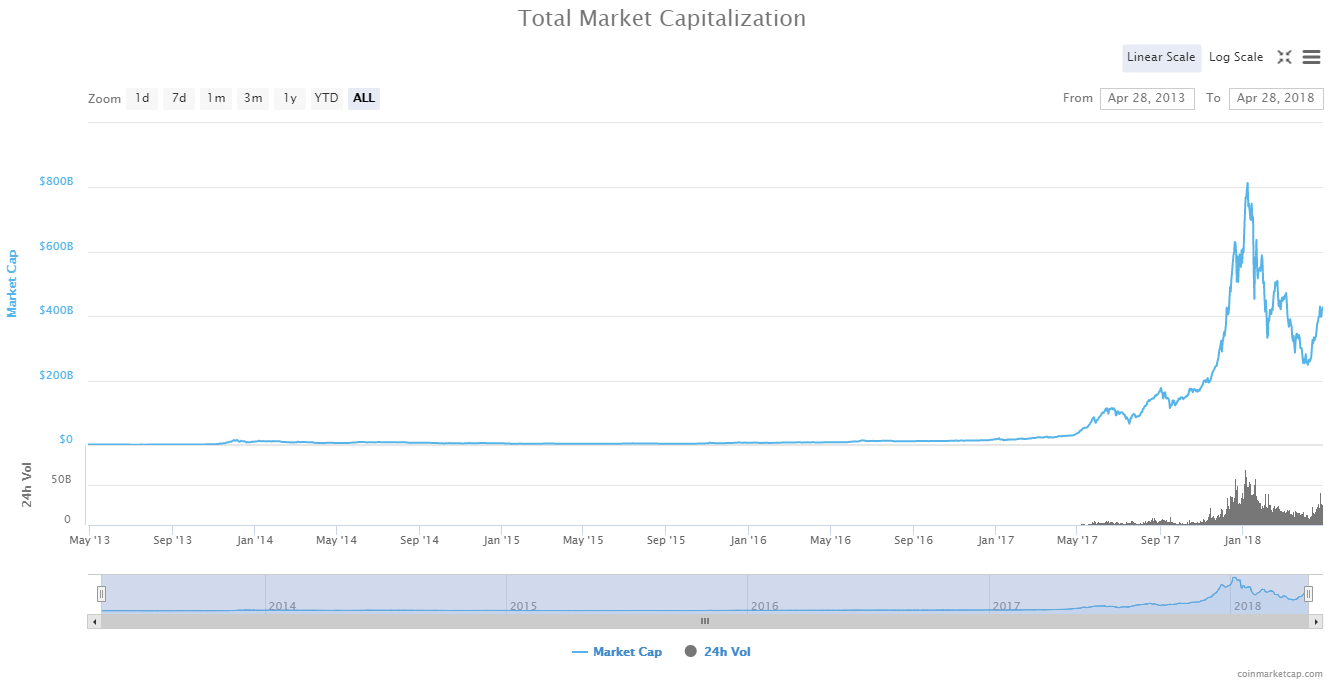
\includegraphics[width=\textwidth,height=\textheight,keepaspectratio]{CryptoMarketCap}
			\captionof{figure}{Capitalizzazione di mercato delle criptovalute - Aprile 2018}
		\end{center}

	\subsection{Tipi di Criptovalute}
		\begin{itemize}
			\item Ci sono al mondo \href{https://coinmarketcap.com/all/views/all/}{più di 1.000 criptovalute} 
			\cite{coinmarketcapAll}	esistenti al momento (chiamate ``altcoin''); 
			con 600 di queste aventi una capitalizzazione di mercato superiore a \$100.000.
			\item Mentre il prezzo di bitcoin ha generalmente sempre seguito un trend rialzista, nei primi del 2018, 
			il prezzo di bitcoin è sceso leggermente,
			\href{https://www.cnbc.com/2018/02/05/bitcoin-price-drops-below-8000-over-60-billion-wiped-off-cryptocurrencies.html}{raggiungendo un minimo di \$8,000} 
			\cite{cnbcBitcoinPriceSurge}
			mentre notizie di regolamentazioni ferree in materia arrivavano dalla Cina e dalla Corea del Sud.
			Il prezzo del bitcoin è anche sceso a seguito dell'annuncio del
			\href{http://www.latimes.com/business/la-fi-bitcoin-sec-registration-20180307-story.html}{blocco della SEC} 
			\cite{laTimes}
			negli exchange di criptovalute dopo che Binance
			\href{https://www.ft.com/content/58a32050-22aa-11e8-add1-0e8958b189ea}{ha ammesso di esser stato hackerato}
			\cite{ftBinanceHack}.
			\item La quota di mercato di bitcoin è scesa dall'81\% di Giugno 2016 al 41\% di Giugno 2017, tuttavia
			il prezzo di bitcoin è continuato a salire.
			\item Nell'Agosto 2017 la capitalizzazione di mercato di ethereum era attorno \$28 miliardi. Ad un certo punto,
			\href{http://www.zerohedge.com/news/2017-05-31/ethereum-forecast-surpass-bitcoin-2018}{alcuni commentatori}
			\cite{zeroHedge}, 
			anticiparono che ethereum avrebbe superato la capitalizzazione di mercato di bitcoin (il 
			\href{https://www.flippening.watch/}{``flippening''} \cite{flippening}). 
			Tuttavia problemi con la tecnologia Ethereum da allora hanno causato il suo prezzo a scendere.
		\end{itemize}
		\begin{center}
			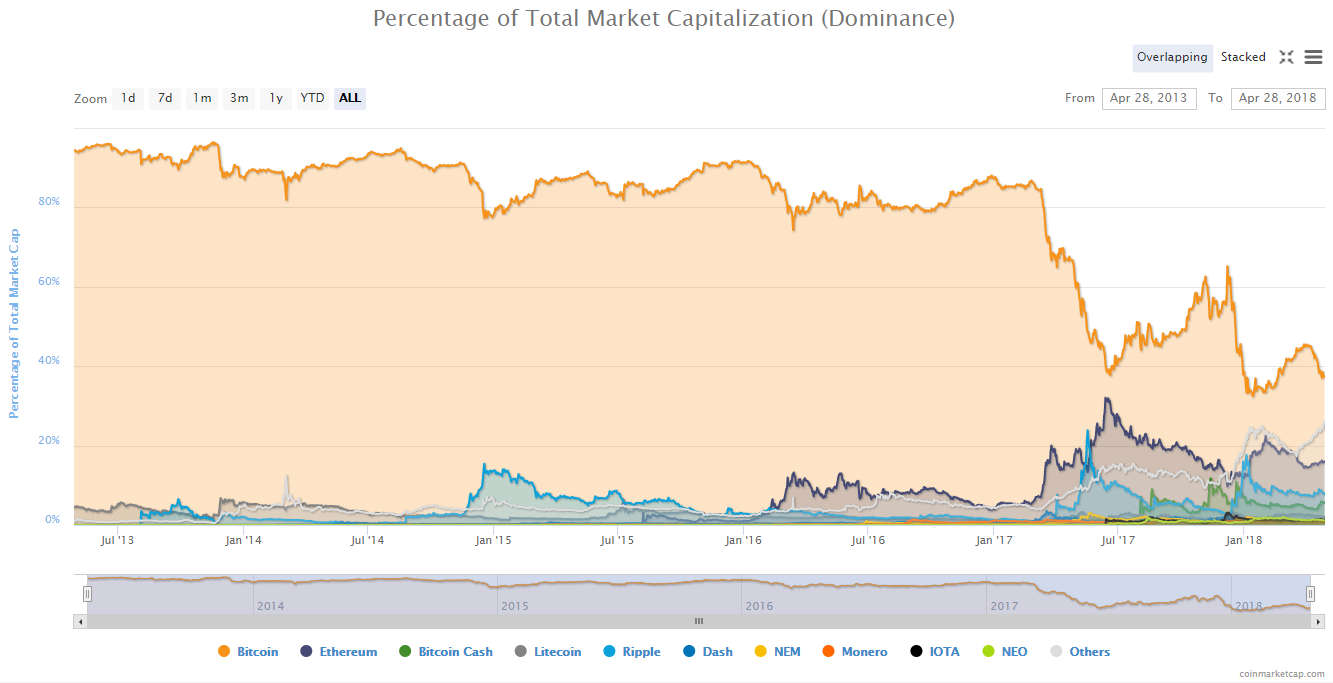
\includegraphics[width=\textwidth,height=\textheight,keepaspectratio]{CryptoMarketDominance}
			\captionof{figure}{Dominio di mercato delle criptovalute - Aprile 2018}
		\end{center}

	\subsection{Investire in Criptovalute}
		\begin{itemize}
			\item Domanda ed offerta contano. Il livello di fornitura di bitcoin continuerà a diminuire fino
			a che bitcoin non raggiunge 21 milioni,
			\href{https://www.coindesk.com/top-10-bitcoin-myths-debunked/}{evento che dovrebbe accadere nel 2140}
			\cite{mythsDebunked}. 
			Similarmente la fornitura di litecoin sarà limitata a 
			\href{https://support.xbtce.info/Knowledgebase/Article/View/152/59/about-litecoin}{84 milioni di untià}
			\cite{ltcLimits}.
			\item Offerte di Valuta Iniziali (Initial Coin Offering) stanno scambiando al momento. Quest'anno
			il CEO di Mozilla Brendon Eich ha raccolto \$35 milioni in una ICO 
			\href{https://techcrunch.com/2017/06/01/brave-ico-35-million-30-seconds-brendan-eich/}{in meno di 30 secondi}
			\cite{techCrunch}, 
			e Bancor Protocol ha raccolto \$153 milioni in	 
			\href{https://www.google.com/search?q=Bancor+Protoco+ico&oq=Bancor+Protocol+ico&gs_l=psy-ab.3..0i13k1l2.253.542.0.578.4.3.0.0.0.0.177.320.0j2.2.0....0...1.1.64.psy-ab..3.1.176.LOjRpj0hKrM}{meno di tre ore}
			\cite{bancorProtocol}.
			\item Progetti correlati alla blockchain hanno raccolto più di 
			\href{https://www.coindesk.com/1-6-billion-all-time-ico-funding-climbs-as-record-500-million-invested-in-july/}{\$1.6 miliari tramite le ICO}
			\cite{coindeskICOAllTimeHigh} 
			ad oggi, mentre i venture capital hanno fornito solamente
			\href{http://my.pitchbook.com/?pbr=14763750}{\$550 milioni} \cite{pitchbook} per compagnie in questa industria.
		\end{itemize}
		\begin{center}
			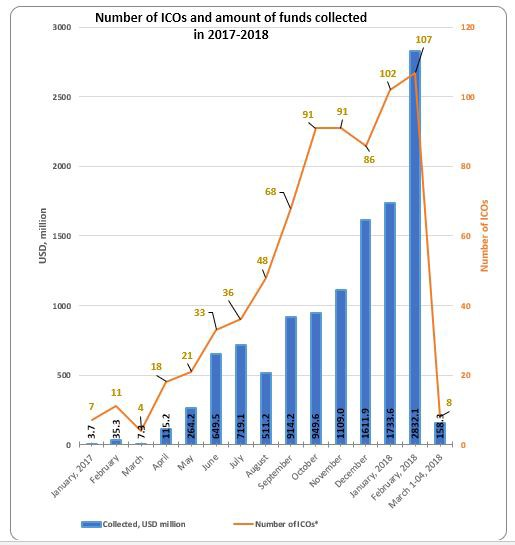
\includegraphics[width=\textwidth,height=\textheight,keepaspectratio]{FundsCollectedICO}
			\captionof{figure}{Fondi raccolti in ICO nel 2017-2018}
		\end{center}

	\subsection{Problemi Irrisolti}
		\begin{itemize}
			\item \textbf{Commerciali}. Mentre gli Stati Uniti hanno fatto una stretta nelle
			attività di regolamentazione, in paesi come la 
			\href{https://techcrunch.com/2013/08/19/germany-recognizes-bitcoin-as-private-money-sales-tax-coming-soon/}{Germania} 
			\cite{techCrunchPrivateMoney}
			ed il \href{http://www.ibtimes.co.uk/hmrc-re-classify-bitcoin-private-money-1432718}{Regno Unito}
			\cite{ibtimesPrivateMoney},
			le criptovalute sono trattate come ``valuta privata'' e non sono soggette a tassazione a parte per l'uso commerciale.
			\item \textbf{Regolatori}. Lo stato di New York ha creato il 
			\href{https://www.wired.com/2014/07/ny_bitcoin/}{sistema BitLicense}
			\cite{wiredNYLicense}, per autorizzare
			compagnie per eseguire attività di cambia valuta virtuale con residenti dello stato di New York.
			A metà 2017 solo tre BitLicense sono state rilasciate ed un numero elevato di richieste sono
			state rimosso o rifiutate. In Asia, dove la richiesta di criptovalute è in ascesa,
			i governi \href{http://fortune.com/2018/01/17/china-bitcoin-cryptocurrency-crackdown/}{Cinese}
			\cite{fortune}
			e \href{https://www.bloomberg.com/news/articles/2017-12-13/south-korea-seeks-measures-to-curb-frenzied-bitcoin-speculation}{Sud Coreano} 
			\cite{bloombergSKBan}
			hanno preso una posizione rigida nella regolamentazione delle criptovalute.
			\item \textbf{Sicurezza}. La 
			\href{https://www.forbes.com/sites/laurashin/2016/12/20/hackers-have-stolen-millions-of-dollars-in-bitcoin-using-only-phone-numbers/#3ac0bf1d38ba}{FTC ha registrato}
			\cite{forbesBitcoinHacking} 
			un aumentare in denuncie di furto di identità di più del 100\% tra il 2013 ed il 2016,
			e Coinbase, il più grande exchange degli Stati Uniti, ha visto un raddoppio nel numero dei furti di 
			account tra Novembre e Dicembre 2016.
		\end{itemize}

\section{Analisi di Mercato Specifica e Proiezione a 5 Anni}
Ripa Exchange alla sua apertura e per tutto il suo primo anno di attività 2019 prevede di avere i 
seguenti numeri operativi:
\begin{itemize}
	\item Utenti Registrati: 	5.000			%(1,600,000 BitFinex, 40,000 TheRockTrading)
	\item Volume 24/ore: 		25 BTC			%(50,000 BTC BitFinex, 100 BTC TheRockTrading)
	\item Volume Mensile: 		750 BTC			%(2,000,000 BTC BitFinex, 5,000 BTC TheRockTrading)
\end{itemize}

Impostata una commissione di transazione del 0,20\% il fatturato per il primo anno di operatività è atteso
essere nell'ordine di 180 BTC mentre il fatturato per gli anni dal secondo al quinto sono previsti nel range 
descritto dal grafico in figura \ref{fig:fiveYearsProhections}.
\begin{center}
	\begin{tikzpicture}
		\begin{axis}[
			symbolic x coords={2019, 2020, 2021, 2022, 2023},
			xtick=data,
			ylabel=BTC,
			xlabel=anno
		]
			\addplot[ybar,fill=azure(colorwheel)] coordinates {
				(2019, 180)
				(2020, 300)
				(2021, 500)
				(2022, 1000)
				(2023, 2000)
			};
			\addplot+ [
				sharp plot, color=silver, mark=diamond
				] coordinates {
				(2019,180) (2020,300) (2021,500) (2022,1000) (2023,2000)
				};			
		\end{axis}	
	\end{tikzpicture}
	\captionof{figure}{Proiezione di fatturato a 5 anni}
	\label{fig:fiveYearsProhections}
\end{center}

A seconda del valore dei fondi raccolti alla chiusura della ICO di RipaEX da 1 a 9 ulteriori Ripa Exchange
sono previsti in apertura nel biennio 2019-2020 allargando l'uso del codice di Ripa Exchange e l'uso del token
XPX associato a Ripa Blockchain. Considerando il dato di previsione a cinque anni per ogni singola istanza
di Ripa Exchange.

\section{Economia del Token XPX}
Come spiegato in sezione \ref{sec:theRipaBlockchain} Ripa Blockchain avrà il suo token nativo XPX (simbolo \PHP)
che servirà ai seguenti scopi:
\begin{enumerate}
	\item per listare nuove valute nell'exchange
	\item per pubblicizzare nuovi progetti
	\item per comprare gadget RipaEx nello store RipaEx Store
	\item per pagare per l'acquisto di beni e servizi in rivenditori autorizzati tramite il RipaEx POV (Punto di Vendita)
	\item per condividere liquidità tra tutti gli exchnage della rete Ripa
\end{enumerate}
E' nostro obbiettivo principale che l'economia del token XPX sia in salute per tutta la durata del progetto RipaEx,
per tale ragione applicheremo strategie di economia di mercato\footnote{Come la distruzione dei token non coperti
da fondi di ICO} all'economia dei token XPX per far si che il presso sia in costante ascesa per tutta la durata
del progetto ed oltre.

%----------------------------------------------------------------------------------------
%	CHAPTER 7: Conclusion
%----------------------------------------------------------------------------------------

\chapterimage{chapter_head_7_LosAngeles.jpg} % Chapter heading image
\chapter{Team e Conclusioni}
\section{Team}
\begin{tcbraster}[raster columns=1,raster rows=1,raster height=0.4cm,
	valign=center, halign=center,
	enhanced,size=small,sharp corners,colframe=azure(colorwheel),coltext=white,
	colback=azure(colorwheel),fit algorithm=hybrid* ]
	\tcboxfit{}
\end{tcbraster}
\begin{tcbraster}[raster columns=2,raster rows=4,raster height=10cm,
	valign=center, halign=left,
	enhanced,size=small,sharp corners,colframe=silver,coltext=black,
	colback=silver,fit algorithm=hybrid* ]
	\tcboxfit{\tcbfontsize{0.8} \textbf{Giovanni Silvestri @ BitNow}\\
	\textsc{Membro Foundatore e CEO}\\
	10+ anni di esperienza in IT,\\
	4+ anni di esperienza in criptovalute,\\
	2+ anni di esperienza in finanza,\\
	Locazione: Treviso (TV), Italia\\
	\href{https://bitcointalk.org/index.php?action=profile;u=497151;sa=summary}{\faBitcoin}
	\href{https://www.linkedin.com/in/zackko/}{\faLinkedin}
	\href{https://t.me/BitNow}{\faSend}}
	\tcboxfit{\tcbfontsize{0.8} \textbf{Antonello Arena @Darkital}\\
	\textsc{Membro Fondatore e CFO}\\
	10+ anni di esperienza in economia e finanza,\\
	4+ anni di esperienza in criptovalute,\\
	Locazione: Potenza (PO), Italia\\
	\href{https://www.linkedin.com/in/antonello-arena-a26b60b7/}{\faLinkedin}
	\href{https://t.me/darkital}{\faSend}}

	\tcboxfit{\tcbfontsize{0.8} \textbf{Giorgio Isola @isolagio}\\
	\textsc{Membro Fondatore e CDO}\\
	10+ anni di esperienza in design,\\
	4+ anni di esperienza in criptovalute,\\
	Locazione: Milano (MI), Italia\\
	\href{https://bitcointalk.org/}{\faBitcoin}
	\href{https://www.linkedin.com/}{\faLinkedin}
	\href{https://t.me/isolagio}{\faSend}}
	\tcboxfit{\tcbfontsize{0.8} \textbf{Proponi il tuo NOME qui}\\
	\textsc{CSO}\\
	3+ anni di esperienza in IT networking,\\
	1+ anni di esperienza in sicurezza informatica,\\
	1+ anni di esperienza in finanza e/o criptovalute,\\
	Locazione: \\
	\href{https://bitcointalk.org/}{\faBitcoin}
	\href{https://www.linkedin.com/}{\faLinkedin}
	\href{https://t.me/}{\faSend}}

	\tcboxfit{\tcbfontsize{0.8} \textbf{Luca Dordolo @gavrilobtc}\\
	\textsc{Advisor}\\
	5+ anni di esperienza in scambio, advisoring e gestione criptovalute\\
	Locazione: Udine (UD), Italia\\
	\href{https://bitcointalk.org/index.php?topic=327894.0}{\faBitcoin}
	\href{http://www.gavrilobtc.it/}{\faRss}
	\href{https://t.me/gavrilobtc}{\faSend}}
	\tcboxfit{\tcbfontsize{0.8} \textbf{Proponi il tuo NOME qui}\\
	\textsc{Advisor}\\
	5+ anni di esperienza in scambio, advisoring e gestione\\
	5+ anni di esperienza in criptovalute,\\
	Locazione: \\
	\href{https://bitcointalk.org/}{\faBitcoin}
	\href{https://www.linkedin.com/}{\faLinkedin}
	\href{https://t.me/}{\faSend}}

	\tcboxfit{\tcbfontsize{0.8} \textbf{Proponi il tuo NOME qui}\\
	\textsc{developer}\\
	3+ anni di esperienza in programmazione,\\
	1+ anni in Ruby on Rails,\\
	1+ anni di esperienza in finanza e/o criptovalute,\\
	Locazione: \\
	\href{https://bitcointalk.org/}{\faBitcoin}
	\href{https://www.linkedin.com/}{\faLinkedin}
	\href{https://t.me/}{\faSend}}
	\tcboxfit{\tcbfontsize{0.8} \textbf{Proponi il tuo NOME qui}\\
	\textsc{developer}\\
	3+ anni di esperienza in programmazione,\\
	1+ anni in Ruby on Rails,\\
	1+ anni di esperienza in finanza e/o criptovalute,\\
	Locazione: \\
	\href{https://bitcointalk.org/}{\faBitcoin}
	\href{https://www.linkedin.com/}{\faLinkedin}
	\href{https://t.me/}{\faSend}}

	\tcboxfit{\tcbfontsize{0.8} \textbf{Proponi il tuo NOME qui}\\
	\textsc{Technical support}\\
	1+ anni di esperienza in supporto tecnico/call center,\\
	1+ anni di esperienza in finanza e/o criptovalute,\\
	Locazione: \\
	\href{https://bitcointalk.org/}{\faBitcoin}
	\href{https://www.linkedin.com/}{\faLinkedin}
	\href{https://t.me/}{\faSend}}
	\tcboxfit{\tcbfontsize{0.8} \textbf{Proponi il tuo NOME qui}\\
	\textsc{Technical support}\\
	1+ anni di esperienza in supporto tecnico/call center,\\
	1+ anni di esperienza in finanza e/o criptovalute,\\
	Location: \\
	\href{https://bitcointalk.org/}{\faBitcoin}
	\href{https://www.linkedin.com/}{\faLinkedin}
	\href{https://t.me/}{\faSend}}

	\tcboxfit{\tcbfontsize{0.8} \textbf{Freewillynow}\\
	\textsc{community manager America}\\
	2+ anni di esperienza in moderazione delle comunità,\\
	5+ anni di esperienza criptovalute,\\
	Locazione: Paesi Bassi\\
	\href{https://t.me/freewillynow}{\faSend}}
	\tcboxfit{\tcbfontsize{0.8} \textbf{OnlyTrifiz}\\
	\textsc{community manager EMEA 1/2}\\
	2+ anni di esperienza in moderazione delle comunità,\\
	5+ anni di esperienza in finanza e/o criptovalute,\\
	Locazione: Italia\\
	\href{https://bitcointalk.org/index.php?action=profile;u=993136}{\faBitcoin}
	\href{https://www.linkedin.com/in/simone-trifiletti/}{\faLinkedin}
	\href{https://t.me/OnlyTrifiz}{\faSend}}

	\tcboxfit{\tcbfontsize{0.8} \textbf{Bitmyst}\\
	\textsc{community manager EMEA 2/2}\\
	2+ anni di esperienza in moderazione delle comunità,\\
	5+ anni di esperienza in criptovalute,\\
	Locazione: Italia\\
	\href{https://t.me/Bitmyst}{\faSend}}
	\tcboxfit{\tcbfontsize{0.8} \textbf{Warren Rogers @wazzy}\\
	\textsc{community manager Africa - Asia}\\
	2+ anni di esperienza in moderazione delle comunità,\\
	5+ anni di esperienza in criptovalute,\\
	5+ anni di esperienza in IT,\\
	Location: Repubblica Ceca\\
	\href{https://www.linkedin.com/in/warren-rogers-8721a069/}{\faLinkedin}
	\href{https://t.me/Wazzy}{\faSend}}

	\tcboxfit{\tcbfontsize{0.8} \textbf{Goose}\\
	\textsc{Delegate}\\
	1+ anni di esperienza come delegato DPoS,\\
	8+ anni di esperienza in finanza e/o criptovalute,\\
	Locazione: Stati Uniti\\
	\href{https://bitcointalk.org/index.php?action=profile;u=1122579}{\faBitcoin}
	\href{https://t.me/Delegate_Goose}{\faSend}}
	\tcboxfit{\tcbfontsize{0.8} \textbf{Pimoussefrnl}\\
	\textsc{Delegate}\\
	4+ anni di esperienza come delegato DPoS,\\
	\href{https://t.me/pimoussefrnl}{\faSend}}

	\tcboxfit{\tcbfontsize{0.8} \textbf{Bluedragon}\\
	\textsc{Delegate}\\
	2+ anni di esperienza come delegato DPoS,\\
	5+ anni di esperienza in marketing,\\
	Locazione: Regno Unito\\
	\href{https://t.me/bluedragon555}{\faSend}}
	\tcboxfit{\tcbfontsize{0.8} \textbf{Proponi il tuo NOME qui}\\
	\textsc{Delegate}\\
	1+ anni di esperienza come delegato DPoS,\\
	1+ anni di esperienza in finanza e/o criptovalute,\\
	Locazione: \\
	\href{https://bitcointalk.org/}{\faBitcoin}
	\href{https://www.linkedin.com/}{\faLinkedin}
	\href{https://t.me/}{\faSend}}
\end{tcbraster}

\section{Raccomandazioni}
Se state pianificando di avviare il vostro crypto asset marketplace siete invitati a seguire la seguente
procedura per eseguire un piano di successo nell'ecosistema Ripa:
\begin{enumerate}
	\item Inoltrate il vostro proposal al Ripa Community Fund nel sito ufficiale\footnote{Disponibile dopo Marzo 2019}
	oppure contattando il Team Ripa direttamente nei canali social indicati di seguito
	\item Ottenete i fondi necessari all'avvio da RCF, da Venture Capital o tramite ICO 
	\item Decidete le specifiche funzionali dell'exchange
	\item Implementate l'exchange
	\item Aprite al pubblico
\end{enumerate}

Seguendo la procedura sopra riportata siete garantiti di avere alte possibilità di avviare un exchange di 
successo per il quale avete il codice sorgente e che genererà fatturato per la vostra attività 
imprenditoriale nei 5 anni a seguire.

Non ci stancheremo mai di ripetere che se la vostra intenzione è di aprire un exchange FIAT $\Leftrightarrow$ CRYPTO 
dovete focalizzarvi in prima istanza in conformità con la legislazione AML/KYC del Paese di incorporazione
e trovare un partner bancario con cui lavorare. Le Autorità Finanziarie Locali possono darvi supporto tecnico
con le regole ed i regolamenti e le fondazioni Bitcoin locali possono aiutarvi per personalizzare le vostre
operazioni di cambia valuta virtuale per eseguire scambi focalizzati sugli interessi dei clienti nel Paese di avvio
attività, romuovendo ambienti \textit{cryptocurrency friendly} nell'area di interesse.\\

Ricordate che \textbf{\textsc{eseguire operazioni di cambiavaluta virtuale è difficile}} per questo vi forniamo di tutti
gli strumenti per avviare la vostra attività imprenditoriale di cui avete bisogno: codice sorgente,
liquidità e finanziamenti saranno a voi disponibili dal giorno 1 di avvio delle vostre operazioni di cambiavaluta virtuale
in modo tale che voi possiate focalizzarvi nel fornire supporto di livello platino ai vostri clienti, ricercare
conformità legislativa e patnership con istituzioni finanziarie per il successo delle vostra attività.

\textsc{Il vostro successo è il successo della rete Ripa} e vogliamo raggiungere questo con duro lavoro e le più 
avanzate tecnologie dell'industria delle valute virtuali per \textsc{TE} e per la soddisfazione dei clienti della
rete Ripa.

\newpage
\section{Social}
\label{sec:social}
Enrate nel nostro \href{https://t.me/ripaex}{canale Telegram} liberamente e dateci feedback sul whitepaper di RipaEx.\\

Per essere parte della comunità e per imparare meglio cosa facciamo:
\begin{itemize}
	\item \textbf{Visitate il nostro sito web} \href{https://www.ripaex.io}{\faHome \hspace{0.2cm} www.ripaex.io} 
	\item \textbf{Entrate in Telegram} \href{https://t.me/ripaex}{\faSend \hspace{0.2cm} t.me/ripaex}
	\item \textbf{Entrate in Slack} \href{https://join.slack.com/t/ripaex/shared_invite/enQtMzM4NzUwNjU4OTQ0LTY3MDJmMTdhYTNlZjJlNGUxNzM1YjUwYjgyYjZlMDJmOTg3NTIzNThmNTYyMGQ3ODBkOTRmYzk3Y2Y4MzBkOTY}{\faSlack \hspace{0.2cm} ripaex.slack.com}
	\item \textbf{Seguiteci in Twitter} \href{https://twitter.com/ripaex}{\faTwitter \hspace{0.2cm} twitter.com/ripaex}
	\item \textbf{Seguiteci in Facebook} \href{https://www.facebook.com/ripaex}{\faFacebook \hspace{0.2cm} www.facebook.com/ripaex}
	\item \textbf{Inviateci un'e-mail} \href{mailto:info@ripaex.io}{\faInternetExplorer \hspace{0.2cm} info@ripaex.io}
\end{itemize}
%----------------------------------------------------------------------------------------
%	CHAPTER 8: Legal
%----------------------------------------------------------------------------------------

\chapterimage{chapter_head_8_KualaLumpur.jpg} % Chapter heading image

\chapter{\textsc{Note Legali}}
\begin{scriptsize}
	{\scshape
		\section{\textsc{Premessa}}
		Per favore leggete questa sezione con attezione ed, in caso di dubbi, consultatevi con il vostro legale di fiducia
		\section{\textsc{Statuto di Responsabilità}} 
		Il whitepaper RipaEx è stato approvato dalla maggioranza del Ripa Founder Team.	I direttori, i membri 
		dell'esecutivo ed i membri della gestione del progetto RipaEx hanno accettato piena responsabilità
		per le affermazioni di questo whitepaper ed assicurato,	in buona fiducia, che quanto scritto non contiene false 
		informazioni od ommissioni che possano compromettere la riuscita di successo del progetto od 
		il vantaggio che gli INVESTITORI del progetto possono ricevere se intendono supportare il progetto.
		\section{\textsc{Informazioni Importanti}}
		\begin{enumerate}
			\item Il progetto RipaEx e le valute XPX non sono da considerarsi security in nessuna giurisdizione.
			Il whitepaper dove spiega RIPA TEC non costituisce ne intende essere un prospetto o proposta 
			avente valore legale in nessuna forma in nessuno stato di applicazione, e non intende essere 
			un'offerta di security oppure un sollecito ad investire in security in nessuna giurisdizione.
			\item Questo whitepaper non è, e non deve essere inteso, come una raccomandazione dei creatori 
			dello stesso ad investire nel progetto. Questo whitepaper non sostituisce, e non deve essere 
			considerato come, un'analisi indipendente di mercato e/o una valutazione commerciale. 
			Ogni ricevente del whitepaper deve eseguire in maniera autonoma indagini di mercato e valutazioni atte
			a considerare in termini prudenziali l'investimento in termini di rischio, possibilità personali 
			ed ogni complicazione nel potenziale economico dell'investimento in questo progetto.
			\item La distribuzione di documentazione relativa a questo whitepaper, l'analisi ed ogni altra 
			informazione riguardo RIPA TEC potrebbero essere proibite nello Stato o nella giurisdizione di Vostra residenza.
			Chiunque decida di distribuire documentazione relativa a RIPA TEC deve accertasi, con i propri 
			consiglieri legali, la legittimità della distribuzione di questa documentazione nel Paese di residenza o domicilio. 
			RipaEx declina ogni responsabilità per la distribuzione dei documenti da essa prodotti in Paesi dove 
			la distribuzione degli stessi è vietata. 
			\item Nessuna persona è presa, invitata o richiesta a forza ad entrare in legame commerciale, legale o di
			investimento contrattuale nei rispetti di RIPA TEC o di investimenti futuri nel progetto RipaEx.
			\item Per quanto concerne l'acquisto delle valute derivate dall'investimento in RIPA TEC, ogni utente ha piena
			libertà commerciale e pubblicictaria di qualsiasi altro scambio privato in materia legiferato dalla possibilità
			di acquisto/vendita nello Stato di sua residenza e/o domicilio.
			\item Nessuna autorità legale ha esaminato o approvato questa documentazione, documentazione che è stata scritta
			usando come esempio la legge europea che governa la pubblicazione di testi e documenti nel momento di scrittura.
			Questa documentazione potrebbe non essere conforme alla legge dello stato da cui gli INVESTITORI provengono,
			in tale caso un avvocato deve essere consultato per ottenere informazioni aggiuntive in riguardo la legalità
			di RIPA TEC e le leggi internazionali alla quali RIPA TEC deve essere sottomessa una volta lanciata.
			\item Il rischio associato ad investimenti finanziari, al valore delle valute, alla finalizzazione del progetto
			saranno chiaramente spiegati nella sezione ``Rischi'' di questo documento.
			\item La riproduzione, modifica o distribuzione di questo documento per fini commerciali, criminali o per ogni
			altro fine non specificatamente indicato in questo documento stesso è strettamente vietata.
			\item Accettando questo whitepaper (considerato come documento scaricabile al sito https://ripaex.io od in
			ogni altro modo di accesso al whitepaper) ogni destinatario ricevente il whitepaper stesso accetta i termini
			e le condizioni fornite dal documento stesso.
			Il destinatario concorda e conferma inoltre:
			\begin{description}
				\item[A)] di trattare tutte queste informazioni in modo confidenziale;
				\item[B)] di aver ricevuto questo documento e/o comprato la valuta XPX in maniera legittima nello stato o 
				giurisdizione di residenza o domicilio del soggetto; 
				\item[C)] di essere conforme a tutte le leggi applicabili a questo whitepaper ed all'acquisto ti valuta XPX; 
				\item[D)] gli esecutori dello scambio, i loro direttori, i loro impiegati, i fondatori del progetto, i loro
				consiglieri legali non sono e non saranno in violazione della legge nello Stato o giurisdizione nella quale
				il ricevente del whitepaper e/o il compratore di valuta XPX risiede o domicilia. Inoltre, essi, non avranno
				alcuna responsabilità in caso la consegna del whitepaper o la vendita di valuta XPX diventi illegale, 
				inapplicabile, vietata o proibita nello Stato o giurisdizione del ricevente;
				\item[E)] di essere consapevole che l'offerta di valuta XPX, la loro vendita, il loro trasferimento od altro
				ad esse correlato è in accordo diretto od indiretto con le legge relativa in materia di cambia valuta virtuale
				e tutte le leggi ad essa applicabili;
				\item[F)] di avere conoscenza ed esperienza sufficienti in materia finanziaria e commerciale da essere in grado 
				di valutare il merito ed il rischio dell'acquisto di valuta XPX e di essere in grado e di avere la volontà di
				accertare il merito ed il rischio per ciò che concerne l'acquisto ed il possesso di valuta XPX nello Stato o 
				giuristizione di residenza o domicilio;
				\item[G)] di acquistare valuta XPX per se stesso/se stessa e non per terze parti;
				\item[H)] di accettare e confermare che la valuta emessa da RipaEx non è classificabile o interpretabile come:
				(I) un tipo di valuta se non valuta virtuale;
				(II) bond, azione societaria o azione emessa da persona fisica o giuridica;
				(III) diritto, opzione o strumento derivato relativo a bond o azioni;
				(IV) il diritto di assicurarsi un profitto o di evitare perdite;
				(V) unità in uno schema di investimento qualsiasi;
				(VI) unità in un trust di qualsiasi tipo;
				(VII) qualsiasi forma di derivato;
				(VIII) qualsiasi altra forma di garanzia o tipologia di security..
				\item[I)] di essere consapevole che le informazioni contenute in questo whitepaper potrebbero essere incomplete e/o
				modificate in un secondo tempo;
				\item[J)] di essere completamente informato e consapevole di tutti gli aspetti in relazione all'acquisto, alla vendita
				ed al possesso di valuta XPX in qualsiasi forma anche quelle che non sono direttamente indicate in questo whitepaper,
				ma che potrebbero essere dedotte da una persona informata sui problemi e le complicazioni in materia di valute virtuali 
				e nello specifico per ciò che riguarda Bitcoin, Ethereum e/o altre tipologie di valute virtuali e conferma in maniera
				irrevocabile ed univoca che Lui o Lei comprende le operazioni, il funzionamento, l'uso, il salvataggio, il
				meccanismo di trasmissione ed altro materiale che riguarda le valute virtuali, il software basato sulla tecnologia
				blockchain, i wallet di valuta virtuale e gli smart contract;
			\end{description}
			\item Questo documento può contenere informazioni storiche, stime o report che sono stati presi dalle fonti citate in 
			questo documento stesso o altri in relazione a RIPA TEC, materiale ricercato dal fondatore del progetto o da altri 
			fondatori dello stesso. Nessuna affermazione viene fatta o garantita in riguardo l'accuratezza o la completezza
			delle informazioni, stime o report in questo documento o in documenti scritti da terze parti e correlati dallo stesso.
			\item Questo documento include ``dichiarazioni previsionali''. Tali affermazioni riguardano, a parte altre, la discussione
			delle strategie di business di RipaEx, le attese riguardo la sua posizione nel mercato, operazioni future, profitto,
			responsabilità, asset e posizioni finanziarie. Tutte queste affermazioni sono basate su stime ed ipotesi fatte dai 
			fondatori del progetto i quali, anche se considerate ragionevoli, sono soggetti a rischi ed incertezze causati da eventi
			reali e che i risultati dei fondatori del progetto potrebbero essere diversi da quanto anticipato o indicato dalle 
			dichiarazioni fatte e nessuna garanzia esplicita od implicita viene data su tali dichiarazioni. Alla luce di queste e 
			di altre incertezze l'inclusione di una dichiarazione previsionale all'interno di questo documento o whitepaper non
			deve essere considerata come una rappresentazione o garanzia di RIPA TEC in ogni caso.
			\item Questo documento ed il suo contenuto sono strettamente confidenziali e le informazioni contenute in esso sono
			fornite ai riceventi concordando implicitamente il fatto che le informazioni in esso sono strettamente confidenziali.
			Conseguenza di ciò tale documento, il suo contenuto ed ogni altra informazione a disposizione del ricevente deve essere
			tenuto in sicurezza. In caso di rottura della garanzia di confidenzialità o nel caso ci siano sospetti che questa 
			confidenzialità non sia più in essere, i fondatori del progetto potrebbero, a loro discrezione, richiedere un indennizzo
			agli esecutori del progetto in base alle leggi vigenti. L'esecutore del progetto ha il diritto di recuperare i costi,
			le spese, e le perdite intercorse in caso di violazione suddetta da parte di un soggetto criminale. Per eliminare
			ogni ragionevole dubbio, la garanzia di confidenzialità è resa attribuibile al ricevente, al consulente professionale,
			all'amministratore, al dipendente, od a qualsiasi altra persona coinvolta nel progetto come l'esecutore dello stesso
			o qualsiasi altra persona raggiunta dai benefici del progetto RipaEx.
			\item RipaEx non garantisce e non fornisce rimborso ai partecipanti. Tutto ciò che è scritto in questo whitepaper
			è basato su indagini di mercato, analisi commerciali ed analisi tecnice eseguite da professionisti del settore i quali
			potrebbero aver fatto errore che potrebbero portare ad una perdita finanziaria. Il valore della valuta XPX non è 
			garantito di salire all'infinito ed i termini di riacquisto della valuta sono definiti in questo documento.
			\item RipaEx garantisce tutto l'impegno fisico e mentale per il raggiungimento degli obbiettivi descritti in questo
			whitepaper tuttavia non si assume la responsabilità in caso di non raggiungimento degli stessi per cause di forza maggiore
			tipo eventi di terze parti, cambio di legislazione, eventi catastrofici che potrebbero variare gli obbiettivi indicati,
			portare alla cancellazione degli stessi o portare alla chiusura anticipata del progetto.
			\item La sezione Rischi è organizzata in modo da incorporare, assieme al disconoscimento legale, un tipo di avvertimento
			a tutti gli INVESTITORI del progetto in riguardo dei rischi correlati all'attività finanziaria nelle valute virtuali ed
			all'investimento in RIPA TEC.
		\end{enumerate}		
	}
\end{scriptsize}

%----------------------------------------------------------------------------------------
%	BIBLIOGRAPHY
%----------------------------------------------------------------------------------------
\chapterimage{chapter_head_9_Milan.jpg} % Chapter heading image
\nocite{*}
\printbibliography[title={Riferimenti}]
\addcontentsline{toc}{chapter}{\textcolor{trolleygrey}{Riferimenti}}
%------------------------------------------------
\newpage
~\vfill
\thispagestyle{empty}
%\begin{center}
%	\noindent Pagina lasciata intenzionalmente bianca
%\end{center}
\chapterimage{chapter_head_10_Frankfurt.jpg} % Chapter heading image
\listoftodos
\end{document}
